\documentclass[a4paper,11pt,report]{ltjsbook}
\usepackage{fancyhdr}
\usepackage[dvipdfmx]{graphicx} % for \includegraphics[width=3cm]{sample.eps}
\usepackage{times} % use Times Font instead of Computer Modern
\usepackage{hyperref}
\setcounter{tocdepth}{3}
\setcounter{page}{-1}
\usepackage{fontspec}
\usepackage{float}
\usepackage{pdflscape}

\usepackage[dvipsnames]{xcolor}
\usepackage{titlesec}
\definecolor{MSBlue}{rgb}{.204,.353,.541}
\definecolor{MSLightBlue}{rgb}{.31,.506,.741}
% Define a new fontfamily for the subsubsection font
% Don't use \fontspec directly to change the font
%\newfontfamily\subsubsectionfont[Color=MSLightBlue]{Times New Roman}
% Set formats for each heading level
\titleformat{\chapter}[display]{\bfseries\HUGE\color{MSBlue}}
{\filleft\Huge\colorbox{MSBlue}{\textcolor{white}{\thechapter}}}
{-0.23em}
{\titlerule\vspace{1ex}\filright}
[\vspace{1ex}\titlerule]

\titlespacing*{\chapter}{0pt}{0pt}{30pt}
\titleformat{\section}[block]
            {\Large\bfseries\sffamily\color{MSLightBlue}}
            {\thesection}
            {1em}{}
            [\titlerule]
\titleformat*{\subsection}{\large\bfseries\sffamily\color{MSLightBlue}}
\titleformat*{\subsubsection}{\itshape\color{MSLightBlue}}

\renewcommand{\chaptermark}[1]{\markboth{#1}{}}

\pagestyle{fancy}
\rhead{\leftmark}
\lhead{\rightmark}

\hypersetup{
    colorlinks,
    pdfencoding=auto,
    citecolor=Sepia,
    filecolor=Sepia,
    linkcolor=Sepia,
    urlcolor=Sepia
}

%\setlength{\oddsidemargin}{0.1in}
%\setlength{\evensidemargin}{0.1in} 
%\setlength{\topmargin}{0in}
%\setlength{\textwidth}{6in} 
%%\setlength{\textheight}{10.1in}
%\setlength{\parskip}{0em}
%\setlength{\topsep}{0em}

%\newcommand{\zu}[1]{{\gt \bf 図\ref{#1}}}

\usepackage{tikz}
\usepackage{tikzscale}
\usetikzlibrary{shapes.multipart,positioning}
\usetikzlibrary{arrows}
\usetikzlibrary{arrows.meta}
\usetikzlibrary{positioning}
\usetikzlibrary[graphs]

\usepackage{pgfplots}
\usepackage{ifthen}

\tikzset{
    font=\ttfamily,
    BLOCK/.style={
        draw,
        align=center,
        text height=0.4cm,
        draw=red!50,
        fill=red!20,
        rectangle split, 
        rectangle split horizontal,
        rectangle split parts=#1, 
        
    }
}

\usepackage{environ}
\makeatletter

\newsavebox{\measure@tikzpicture}
\NewEnviron{scaletikzpicturetowidth}[1]{%
  \def\tikz@width{#1}%
  \def\tikzscale{1}\begin{lrbox}{\measure@tikzpicture}%
  \BODY
  \end{lrbox}%
  \pgfmathparse{#1/\wd\measure@tikzpicture}%
  \edef\tikzscale{\pgfmathresult}%
  \BODY
}
\makeatother


\definecolor{ikkonzome}{rgb}	{	0.9961	,	0.7569	,	0.7373	}
\definecolor{ishitake}{rgb}	{	0.9961	,	0.6941	,	0.7059	}
\definecolor{momo}{rgb}	        {	0.9961	,	0.6824	,	0.8039	}
\definecolor{kobai}{rgb}	{	0.9412	,	0.4235	,	0.5569	}
\definecolor{nakabeni}{rgb}	{	0.9451	,	0.2706	,	0.4941	}
\definecolor{sakura}{rgb}	{	0.9333	,	0.8353	,	0.8353	}
\definecolor{arazome}{rgb}	{	0.9725	,	0.7216	,	0.7843	}
\definecolor{usubeni}{rgb}	{	0.8471	,	0.4471	,	0.5451	}
\definecolor{hisame}{rgb}	{	0.7451	,	0.4039	,	0.4039	}
\definecolor{toki}{rgb}	        {	0.9569	,	0.6431	,	0.6353	}
\definecolor{sakuranezumi}{rgb}	{	0.6941	,	0.6039	,	0.6078	}
\definecolor{sango}	{rgb}	{	0.8471	,	0.4157	,	0.3725	}
\definecolor{akane}	{rgb}	{	0.7529	,	0.0118	,	0.3451	}
\definecolor{choshun}{rgb}	{	0.7490	,	0.5255	,	0.5255	}
\definecolor{karakurenai}{rgb}	{	0.7373	,	0.0118	,	0.2667	}
\definecolor{enji}{rgb}	        {	0.6275	,	0.0863	,	0.3176	}
\definecolor{keshiaka}{rgb}	{	0.6275	,	0.4275	,	0.4275	}
\definecolor{kokiake}{rgb}	{	0.5059	,	0.0706	,	0.2549	}
\definecolor{jinzamomi}{rgb}	{	0.9098	,	0.4549	,	0.4157	}
\definecolor{mizugaki}{rgb}	{	0.7294	,	0.5529	,	0.4784	}
\definecolor{umenezumi}{rgb}	{	0.5882	,	0.3922	,	0.3882	}
\definecolor{suoko}{rgb}        {	0.5843	,	0.2667	,	0.2431	}
\definecolor{akabeni}{rgb}	{	0.8039	,	0.0784	,	0.3725	}
\definecolor{shinshu}{rgb}	{	0.6431	,	0.0353	,	0.0000	}
\definecolor{azuki}{rgb}	{	0.5255	,	0.0235	,	0.0000	}
\definecolor{ginshu}{rgb}	{	0.7490	,	0.2824	,	0.0588	}
\definecolor{ebicha}{rgb}	{	0.4549	,	0.2706	,	0.2627	}
\definecolor{kuriume}{rgb}	{	0.5843	,	0.3804	,	0.4314	}
\definecolor{akebono}{rgb}	{	0.8902	,	0.5961	,	0.4941	}
\definecolor{hanezu}{rgb}	{	0.7882	,	0.5961	,	0.5373	}
\definecolor{sangoshu}{rgb}	{	0.8196	,	0.5059	,	0.4471	}
\definecolor{shozyohi}{rgb}	{	0.7686	,	0.0000	,	0.0000	}
\definecolor{shikancha}{rgb}	{	0.5569	,	0.3294	,	0.1882	}
\definecolor{kakishibu}{rgb}	{	0.6745	,	0.4078	,	0.3333	}
\definecolor{benikaba}{rgb}	{	0.7137	,	0.3373	,	0.2941	}
\definecolor{benitobi}{rgb}	{	0.6196	,	0.3176	,	0.2706	}
\definecolor{benihihada}{rgb}	{	0.5020	,	0.3137	,	0.2353	}
\definecolor{kurotobi}{rgb}	{	0.3176	,	0.2000	,	0.1490	}
\definecolor{benihi}{rgb}	{	0.8235	,	0.4745	,	0.1922	}
\definecolor{terigaki}{rgb}	{	0.8118	,	0.4627	,	0.1804	}
\definecolor{ake}{rgb}	        {	0.7804	,	0.3098	,	0.1725	}
\definecolor{edocha}{rgb}	{	0.6863	,	0.4353	,	0.2941	}
\definecolor{bengara}{rgb}	{	0.6392	,	0.1569	,	0.0196	}
\definecolor{hihada}{rgb}	{	0.5412	,	0.3412	,	0.2353	}
\definecolor{shishi}{rgb}	{	0.8549	,	0.6863	,	0.5961	}
\definecolor{araishu}{rgb}	{	0.9294	,	0.4902	,	0.4549	}
\definecolor{akago}{rgb}	{	0.8118	,	0.5765	,	0.4275	}
\definecolor{tokigaracha}{rgb}	{	0.7922	,	0.5255	,	0.3686	}
\definecolor{otan}{rgb}	        {	0.8157	,	0.4157	,	0.2235	}
\definecolor{komugi}{rgb}	{	0.8157	,	0.6549	,	0.5098	}
\definecolor{rakuda}{rgb}	{	0.6784	,	0.5255	,	0.4118	}
\definecolor{tsurubami}{rgb}	{	0.6275	,	0.4392	,	0.3961	}
\definecolor{ama}{rgb}	        {	0.7765	,	0.6902	,	0.5843	}
\definecolor{nikkei}{rgb}	{	0.7216	,	0.4667	,	0.3725	}
\definecolor{renga}{rgb}	{	0.6902	,	0.3765	,	0.3098	}
\definecolor{sohi}{rgb}   	{	0.8078	,	0.5098	,	0.2078	}
\definecolor{enshucha}{rgb}	{	0.6706	,	0.4275	,	0.1608	}
\definecolor{karacha}{rgb}	{	0.5765	,	0.4235	,	0.1490	}
\definecolor{kabacha}{rgb}	{	0.6353	,	0.3725	,	0.1569	}
\definecolor{sodenkaracha}{rgb}	{	0.5216	,	0.3490	,	0.1373	}
\definecolor{suzumecha}{rgb}	{	0.4745	,	0.3176	,	0.1255	}
\definecolor{kurikawacha}{rgb}	{	0.4078	,	0.2745	,	0.1098	}
\definecolor{momoshiocha}{rgb}	{	0.3490	,	0.2353	,	0.0902	}
\definecolor{tobi}{rgb}	        {	0.4353	,	0.3098	,	0.1412	}
\definecolor{kurumizome}{rgb}	{	0.6667	,	0.5333	,	0.3333	}
\definecolor{kaba}{rgb}	        {	0.8196	,	0.4588	,	0.1294	}
\definecolor{korosen}{rgb}	{	0.5059	,	0.3843	,	0.1608	}
\definecolor{kogecha}{rgb}	{	0.3333	,	0.2549	,	0.1098	}
\definecolor{kokikuchinashi}{rgb}	{	0.8078	,	0.5922	,	0.3490	}
\definecolor{araigaki}{rgb}	{	0.8157	,	0.5529	,	0.3176	}
\definecolor{taisha}{rgb}	{	0.6353	,	0.4196	,	0.2078	}
\definecolor{akashirotsurubami}{rgb}	{	0.8078	,	0.6118	,	0.4157	}
\definecolor{tonocha}{rgb}	{	0.5922	,	0.4039	,	0.2000	}
\definecolor{sencha}{rgb}	{	0.5255	,	0.3529	,	0.1490	}
\definecolor{sharegaki}{rgb}	{	0.8549	,	0.7098	,	0.4863	}
\definecolor{ko}{rgb}	        {	0.9529	,	0.8275	,	0.6627	}
\definecolor{usugaki}{rgb}	{	0.8627	,	0.7294	,	0.5294	}
\definecolor{koji}{rgb}	        {	0.8275	,	0.6039	,	0.2706	}
\definecolor{umezome}{rgb}	{	0.8667	,	0.7373	,	0.4235	}
\definecolor{beniukon}{rgb}	{	0.8549	,	0.5843	,	0.2549	}
\definecolor{chojicha}{rgb}	{	0.5569	,	0.4000	,	0.1098	}
\definecolor{kenpozome}{rgb}	{	0.3059	,	0.2667	,	0.0627	}
\definecolor{biwacha}{rgb}	{	0.7333	,	0.5294	,	0.1922	}
\definecolor{kohaku}{rgb}	{	0.8039	,	0.5961	,	0.2471	}
\definecolor{usuko}{rgb}	{	0.8745	,	0.7373	,	0.4824	}
\definecolor{kuchiba}{rgb}	{	0.8157	,	0.6157	,	0.3216	}
\definecolor{kincha}{rgb}	{	0.7725	,	0.4902	,	0.2000	}
\definecolor{chozizome}{rgb}	{	0.5686	,	0.3961	,	0.1608	}
\definecolor{kitsune}{rgb}	{	0.6392	,	0.4431	,	0.1804	}
\definecolor{hushizome}{rgb}	{	0.5804	,	0.4353	,	0.1608	}
\definecolor{kyara}{rgb}	{	0.4510	,	0.3373	,	0.1255	}
\definecolor{susutake}{rgb}	{	0.4588	,	0.3529	,	0.1176	}
\definecolor{shirocha}{rgb}	{	0.7529	,	0.6588	,	0.4118	}
\definecolor{odo}{rgb}	        {	0.7137	,	0.6039	,	0.3137	}
\definecolor{ginsusutake}{rgb}	{	0.5608	,	0.4745	,	0.2392	}
\definecolor{kigaracha}{rgb}	{	0.7490	,	0.6196	,	0.2745	}
\definecolor{kobicha}	{rgb}	{	0.5020	,	0.4118	,	0.1765	}
\definecolor{usuki}	{rgb}	{	0.8549	,	0.7804	,	0.4275	}
\definecolor{yamabuki}	{rgb}	{	0.9098	,	0.8000	,	0.2039	}
\definecolor{tamago}	{rgb}	{	0.8275	,	0.7412	,	0.3373	}
\definecolor{hajizome}	{rgb}	{	0.7412	,	0.6039	,	0.2431	}
\definecolor{yamabukicha}{rgb}	{	0.7059	,	0.5765	,	0.2275	}
\definecolor{kuwazome}	{rgb}	{	0.6471	,	0.5255	,	0.2118	}
\definecolor{namakabe}	{rgb}	{	0.5569	,	0.4549	,	0.1843	}
\definecolor{kuchinashi}{rgb}	{	0.8078	,	0.7333	,	0.3843	}
\definecolor{tomorokoshi}{rgb}	{	0.7804	,	0.7020	,	0.2941	}
\definecolor{shirotsurubami}{rgb}	{	0.8745	,	0.8235	,	0.5922	}
\definecolor{kitsurubami}{rgb}	{	0.6863	,	0.6039	,	0.2118	}
\definecolor{toou}	{rgb}	{	0.8353	,	0.7725	,	0.4235	}
\definecolor{hanaba}	{rgb}	{	0.8549	,	0.8000	,	0.4941	}
\definecolor{torinoko}	{rgb}	{	0.8431	,	0.8118	,	0.6902	}
\definecolor{ukon}	{rgb}	{	0.8039	,	0.7216	,	0.3059	}
\definecolor{kikuchiba}	{rgb}	{	0.7765	,	0.6667	,	0.2902	}
\definecolor{rikyushiracha}{rgb}{	0.6627	,	0.6471	,	0.4784	}
\definecolor{rikyucha}	{rgb}	{	0.5176	,	0.5176	,	0.2588	}
\definecolor{aku}	{rgb}	{	0.5294	,	0.5059	,	0.4039	}
\definecolor{higosusutake}{rgb}	{	0.4863	,	0.4510	,	0.3059	}
\definecolor{rokocha}	{rgb}	{	0.4157	,	0.4353	,	0.3686	}
\definecolor{mirucha}	{rgb}	{	0.4471	,	0.4471	,	0.3725	}
\definecolor{natane}	{rgb}	{	0.7216	,	0.6863	,	0.3882	}
\definecolor{kimirucha}	{rgb}	{	0.5373	,	0.5059	,	0.2549	}
\definecolor{uguisucha}	{rgb}	{	0.4118	,	0.3882	,	0.1961	}
\definecolor{nanohana}	{rgb}	{	0.9882	,	0.9882	,	0.3804	}
\definecolor{kariyasu}	{rgb}	{	0.8039	,	0.7686	,	0.3882	}
\definecolor{kihada}	{rgb}	{	0.9608	,	0.9137	,	0.2863	}
\definecolor{zoge}	{rgb}	{	0.8863	,	0.8235	,	0.7216	}
\definecolor{wara}	{rgb}	{	0.7882	,	0.7490	,	0.4706	}
\definecolor{macha}	{rgb}	{	0.6235	,	0.6392	,	0.4863	}
\definecolor{yamabato}	{rgb}	{	0.5137	,	0.5176	,	0.4000	}
\definecolor{mushikuri}	{rgb}	{	0.8196	,	0.8000	,	0.6118	}
\definecolor{aokuchiba}	{rgb}	{	0.6275	,	0.6392	,	0.3451	}
\definecolor{hiwacha}	{rgb}	{	0.6784	,	0.6863	,	0.4196	}
\definecolor{ominaeshi}	{rgb}	{	0.8745	,	0.8863	,	0.4039	}
\definecolor{wasabi}	{rgb}	{	0.5922	,	0.6824	,	0.5765	}
\definecolor{uguisu}	{rgb}	{	0.3333	,	0.4118	,	0.0627	}
\definecolor{hiwa}	{rgb}	{	0.7098	,	0.7216	,	0.2392	}
\definecolor{aoshirotsurubami}{rgb}	{	0.5961	,	0.6471	,	0.4471	}
\definecolor{yanagicha}	{rgb}	{	0.5373	,	0.5725	,	0.3529	}
\definecolor{rikancha}	{rgb}	{	0.3333	,	0.4196	,	0.2863	}
\definecolor{aikobicha}	{rgb}	{	0.2706	,	0.3412	,	0.2353	}
\definecolor{koke}	{rgb}	{	0.4941	,	0.5686	,	0.3922	}
\definecolor{miru}	{rgb}	{	0.1529	,	0.3216	,	0.1843	}
\definecolor{sensai}	{rgb}	{	0.1373	,	0.2863	,	0.1608	}
\definecolor{baiko}	{rgb}	{	0.5529	,	0.6157	,	0.3922	}
\definecolor{iwai}	{rgb}	{	0.3059	,	0.4118	,	0.2784	}
\definecolor{hiwamoegi}	{rgb}	{	0.4431	,	0.6824	,	0.2431	}
\definecolor{yanagisusutake}{rgb}	{	0.2039	,	0.3333	,	0.1255	}
\definecolor{urayanagi}	{rgb}	{	0.5843	,	0.6824	,	0.2431	}
\definecolor{usumoegi}	{rgb}	{	0.4824	,	0.6706	,	0.2275	}
\definecolor{yanagizome}{rgb}	{	0.4353	,	0.6000	,	0.2078	}
\definecolor{moegi}	{rgb}	{	0.3020	,	0.5961	,	0.1882	}
\definecolor{aoni}	{rgb}	{	0.1216	,	0.4196	,	0.2431	}
\definecolor{matsuba}	{rgb}	{	0.1098	,	0.3686	,	0.2118	}
\definecolor{usuao}	{rgb}	{	0.5529	,	0.7059	,	0.6118	}
\definecolor{wakatake}	{rgb}	{	0.3843	,	0.6824	,	0.5059	}
\definecolor{yanaginezumi}{rgb}	{	0.5020	,	0.6078	,	0.5490	}
\definecolor{oitake}	{rgb}	{	0.4157	,	0.5412	,	0.4392	}
\definecolor{sensaimidori}{rgb}	{	0.2549	,	0.3882	,	0.2627	}
\definecolor{midori}	{rgb}	{	0.0000	,	0.4824	,	0.0000	}
\definecolor{byakuroku}	{rgb}	{	0.6078	,	0.7333	,	0.6196	}
\definecolor{sabiseiji}	{rgb}	{	0.5333	,	0.6588	,	0.5804	}
\definecolor{rokusho}	{rgb}	{	0.3373	,	0.6039	,	0.4039	}
\definecolor{tokusa}	{rgb}	{	0.2549	,	0.4706	,	0.3922	}
\definecolor{onandocha}	{rgb}	{	0.2039	,	0.3725	,	0.3098	}
\definecolor{aotake}	{rgb}	{	0.1412	,	0.5176	,	0.4353	}
\definecolor{rikyunezumi}{rgb}	{	0.4157	,	0.5686	,	0.5490	}
\definecolor{birodo}	{rgb}	{	0.1059	,	0.4275	,	0.3608	}
\definecolor{mishiao}	{rgb}	{	0.1098	,	0.4588	,	0.3882	}
\definecolor{aimirucha}	{rgb}	{	0.2510	,	0.4000	,	0.3608	}
\definecolor{tonotya}	{rgb}	{	0.3059	,	0.4941	,	0.4392	}
\definecolor{mizuasagi}	{rgb}	{	0.1569	,	0.6745	,	0.6745	}
\definecolor{seji}	{rgb}	{	0.4745	,	0.6588	,	0.5922	}
\definecolor{seheki}	{rgb}	{	0.0588	,	0.5569	,	0.4824	}
\definecolor{sabitetsu}	{rgb}	{	0.0392	,	0.3294	,	0.2784	}
\definecolor{tetsu}	{rgb}	{	0.0627	,	0.3961	,	0.3961	}
\definecolor{omeshicha}	{rgb}	{	0.0667	,	0.4667	,	0.4667	}
\definecolor{korainando}{rgb}	{	0.0588	,	0.3922	,	0.0392	}
\definecolor{minatonezumi}{rgb}	{	0.4549	,	0.6000	,	0.6118	}
\definecolor{aonibi}	{rgb}	{	0.1804	,	0.3725	,	0.3882	}
\definecolor{tetsuonando}{rgb}	{	0.1961	,	0.4118	,	0.4275	}
\definecolor{mizu}	{rgb}	{	0.5451	,	0.7412	,	0.7608	}
\definecolor{sabiasagi}	{rgb}	{	0.4510	,	0.6000	,	0.6000	}
\definecolor{kamenozoki}{rgb}	{	0.7098	,	0.9020	,	0.8902	}
\definecolor{asagi}	{rgb}	{	0.3020	,	0.6784	,	0.7098	}
\definecolor{shinbashi}	{rgb}	{	0.0000	,	0.6000	,	0.6353	}
\definecolor{sabionando}{rgb}	{	0.2392	,	0.3961	,	0.3843	}
\definecolor{ainezumi}	{rgb}	{	0.2235	,	0.4000	,	0.3843	}
\definecolor{ai}	{rgb}	{	0.2039	,	0.3765	,	0.4314	}
\definecolor{onando}	{rgb}	{	0.1843	,	0.3686	,	0.4000	}
\definecolor{hanaasagi}	{rgb}	{	0.2000	,	0.6196	,	0.7098	}
\definecolor{chigusa}	{rgb}	{	0.1922	,	0.5725	,	0.6745	}
\definecolor{masuhana}	{rgb}	{	0.1569	,	0.4667	,	0.5569	}
\definecolor{hanada}	{rgb}	{	0.0039	,	0.4275	,	0.5373	}
\definecolor{noshimehana}{rgb}	{	0.1412	,	0.4235	,	0.5098	}
\definecolor{omeshionando}{rgb}	{	0.1176	,	0.3529	,	0.4235	}
\definecolor{sora}	{rgb}	{	0.1451	,	0.7216	,	0.8039	}
\definecolor{konpeki}	{rgb}	{	0.0902	,	0.5098	,	0.7333	}
\definecolor{kurotsurubami}{rgb}{	0.0627	,	0.3137	,	0.3451	}
\definecolor{gunjo}	{rgb}	{	0.5098	,	0.7882	,	0.9098	}
\definecolor{kon}	{rgb}	{	0.0000	,	0.2000	,	0.4000	}
\definecolor{kachi}	{rgb}	{	0.0000	,	0.1765	,	0.3490	}
\definecolor{ruri}	{rgb}	{	0.0078	,	0.3922	,	0.6510	}
\definecolor{konjo}	{rgb}	{	0.0039	,	0.3137	,	0.5216	}
\definecolor{rurikon}	{rgb}	{	0.0000	,	0.3020	,	0.5020	}
\definecolor{benimidori}{rgb}	{	0.3373	,	0.4588	,	0.6784	}
\definecolor{konkikyo}	{rgb}	{	0.0039	,	0.0667	,	0.4275	}
\definecolor{hujinezumi}{rgb}	{	0.3216	,	0.3686	,	0.6118	}
\definecolor{benikakehana}{rgb}	{	0.2275	,	0.2471	,	0.5882	}
\definecolor{hujiiro}	{rgb}	{	0.4706	,	0.4863	,	0.7059	}
\definecolor{hutaai}	{rgb}	{	0.3137	,	0.3333	,	0.5608	}
\definecolor{hujimurasaki}{rgb}	{	0.4157	,	0.3333	,	0.5686	}
\definecolor{kikyo}	{rgb}	{	0.3529	,	0.3216	,	0.5725	}
\definecolor{shion}	{rgb}	{	0.5137	,	0.4196	,	0.6784	}
\definecolor{messhi}	{rgb}	{	0.2196	,	0.1765	,	0.3098	}
\definecolor{shikon}	{rgb}	{	0.2510	,	0.1961	,	0.3529	}
\definecolor{kokimurasaki}{rgb}	{	0.3098	,	0.2000	,	0.3765	}
\definecolor{usu}	{rgb}	{	0.7294	,	0.6353	,	0.7843	}
\definecolor{hashita}	{rgb}	{	0.6000	,	0.4549	,	0.6706	}
\definecolor{rindo}	{rgb}	{	0.5922	,	0.5137	,	0.7529	}
\definecolor{sumire}	{rgb}	{	0.3882	,	0.2157	,	0.5922	}
\definecolor{nasukon}	{rgb}	{	0.3216	,	0.2235	,	0.4353	}
\definecolor{murasaki}	{rgb}	{	0.3137	,	0.1765	,	0.4824	}
\definecolor{kurobeni}	{rgb}	{	0.2353	,	0.1294	,	0.3059	}
\definecolor{ayame}	{rgb}	{	0.4275	,	0.1569	,	0.5098	}
\definecolor{benihuji}	{rgb}	{	0.6824	,	0.5333	,	0.6667	}
\definecolor{edomurasaki}{rgb}	{	0.3961	,	0.1529	,	0.4392	}
\definecolor{kodaimurasaki}{rgb}{	0.4353	,	0.2863	,	0.4627	}
\definecolor{shikon}{rgb}       {	0.4118	,	0.2549	,	0.3765	}
\definecolor{hatobanezumi}{rgb}	{	0.4235	,	0.3804	,	0.4392	}
\definecolor{budonezumi}{rgb}	{	0.3412	,	0.2196	,	0.3529	}
\definecolor{ebizome}	{rgb}	{	0.4000	,	0.2235	,	0.3882	}
\definecolor{hujisusutake}{rgb}	{	0.2549	,	0.0824	,	0.2471	}
\definecolor{usuebi}	{rgb}	{	0.6549	,	0.4392	,	0.6039	}
\definecolor{botan}	{rgb}	{	0.6706	,	0.0392	,	0.4353	}
\definecolor{umemurasaki}{rgb}	{	0.6667	,	0.3922	,	0.5176	}
\definecolor{nisemurasaki}{rgb}	{	0.3686	,	0.0000	,	0.3216	}
\definecolor{murasakitobi}{rgb}	{	0.3922	,	0.3255	,	0.3529	}
\definecolor{ususuo}{rgb}	{	0.7569	,	0.4000	,	0.5412	}
\definecolor{suo}{rgb}	        {	0.6941	,	0.0627	,	0.4157	}
\definecolor{kuwanomi}{rgb}	{	0.4196	,	0.0549	,	0.2745	}
\definecolor{nibi}{rgb}	        {	0.4549	,	0.4235	,	0.3961	}
\definecolor{benikeshi}{rgb}	{	0.4118	,	0.3804	,	0.3843	}
\definecolor{shironeri}{rgb}	{	0.9843	,	0.9843	,	0.9843	}
\definecolor{shironezumi}{rgb}	{	0.6471	,	0.6588	,	0.6627	}
\definecolor{ginnezumi}{rgb}	{	0.5255	,	0.5490	,	0.5922	}
\definecolor{sunezumi}{rgb}	{	0.4275	,	0.4392	,	0.4392	}
\definecolor{dobunezumi}{rgb}	{	0.2863	,	0.2941	,	0.2941	}
\definecolor{aisumicha}{rgb}	{	0.2078	,	0.2196	,	0.2510	}
\definecolor{binrojizome}{rgb}	{	0.2118	,	0.0824	,	0.0706	}
\definecolor{sumizome}{rgb}	{	0.2706	,	0.2706	,	0.2706	}

\usepackage{listings}
\lstset{
  backgroundcolor=\color{white},   % choose the background color; you must add \usepackage{color} or \usepackage{xcolor}
  basicstyle=\ttfamily,
  commentstyle=\textit,
  frame=trBL,
  keepspaces=true,                 % keeps spaces in text, useful for keeping indentation of code (possibly needs columns=flexible)
  showstringspaces=false,
  numbers=left,
  numbersep=5pt,                   % how far the line-numbers are from the code
  stepnumber=1,
  numberstyle=,
  keywordstyle=\bfseries\color{shinbashi},
 commentstyle=\itshape\color{koke},
  identifierstyle=\color{miru},
  stringstyle=\color{sakuranezumi},
  breakatwhitespace=false,         % sets if automatic breaks should only happen at whitespace
  breaklines=true,                 % sets automatic line breaking
  captionpos=b,                    % sets the caption-position to bottom
  language=C,                 % the language of the code
  rulecolor=\color{black},         % if not set, the frame-color may be changed on line-breaks within not-black text (e.g. comments (green here))
  tabsize=2,	                   % sets default tabsize to 2 spaces
  title=\lstname                   % show the filename of files included with \lstinputlisting; also try caption instead of title
}

\bibliographystyle{acm}

%% タイトル生成用パッケージ(重要)
\usepackage{coins-jp}

\setmainfont{IPAPMincho}
\setsansfont{MigMix 2P}
\setmonofont{Ubuntu Mono}

\usepackage{ulem}

\title{\uline{Offloading device drivers into a hypervisor for separation of concerns}}
%% 著者
\author{米司 伊織}
%% 指導教員
\advisor{加藤和彦}

%% 専攻名 と 年月 (提出年月)
%% 年月は必要に応じて書き替えてください。
\heiseiyear{25}  % 平成の年度
%\majorfield{ソフトウェアサイエンス主専攻}
\majorfield{情報システム主専攻}
%\majorfield{知能情報メディア主専攻}

\usepackage{etoolbox}
\patchcmd{\title}{plain}{empty}{}{}

\begin{document}
\thispagestyle{empty}
\newpage
\thispagestyle{empty}
\begin{minipage}{.8\hsize}
\thispagestyle{empty}
\maketitle
\end{minipage}
\thispagestyle{empty}
\newpage

\thispagestyle{empty}
\vspace*{20pt plus 1fil}
\noindent
%%
%% 論文の概要(Abstract)
%%
\begin{center}
{\Large \bf 要  旨}
\vspace{2cm}
\end{center}

オペレーティングシステムは様々な機能を提供しているが、その中でデバイスドライバの占める開発コストは大きい。そこで本論文では、デバイスドライバを提供する低オーバヘッドのハイパーバイザと、よりシンプルなオペレーティングシステムからなる新しいオペレーティングシステムアーキテクチャ・デザインを提案し、オペレーティングシステムの開発における「関心の分離」を図る。その主要な技法としてDevice Masqueradingについて論じ、本デザインの応用について検討する。また、その評価に際して実際にBitVisorを改変して実装し、性能について実験する。また、さらにネットワーク性能を改善させる方法について議論し評価する。

keywords = {BitVisor, Hypervisor, OS Design, libraryOS, embedded computing, OS noise, open standard, virtio, paravirtual device}


%%%%%
\par
\vspace{0pt plus 1fil}
\newpage

\pagenumbering{roman} % I, II, III, IV 
\tableofcontents
\listoffigures
%\listoftables

\pagebreak \setcounter{page}{1}
\pagenumbering{arabic} % 1,2,3



\chapter{序論}

\section{既存のデバイスドライバの問題点}
近年、オペレーティングシステムのアーキテクチャは転換期をむかえている。その要因として、モバイル・ IoT の普及とともに、オペレーティングシステムの低消費電力化と同時に多様なデバイスに対応しなければならなくなってきているほか、ハイパフォーマンスコンピューティング環境の巨大化によって、よりオペレーティングシステムへの性能要求は高まっている。しかしながら、同時にオペレーティングシステムの開発コストは年々上がっている。その理由として、多様な SoC やデバイスの普及によって、デバイスドライバの開発コストは年々上がっているという点が挙げられる。デバイスドライバは歴史的にオペレーティングシステムの不具合の原因の最たるもので\cite{oserrors}、近年改善されているとはいえ、頻度・件数ともに主要因の一つでありつづけている\cite{faults}。また、オペレーティングシステムの開発コストもデバイスドライバは支配的な存在となっている。このことを示すためにコード行数ベースで比較すると、一例として linux の mainline(1 月 13 日時点での最新)全体に対するデバイスドライバの占める割合は 1884 万行中 1171 万行で 62.2\% となっている。この問題はデバイスドライバが各オペレーティングシステム間で再利用できないことによる。

また、ライブラリ OS の研究がここ数年で盛んになっていて実際に民用においても使われ始めているが、多くのライブラリ OS の実行環境は伝統的なオペレーティングシステムの上に限定されていて、ライブラリ OS のパフォーマンスが引き出せるとは限らない。ライブラリOSではカーネルをライブラリとしてリンクし、実行ファイルでありながら同時にオペレーティングシステムとして動作するもので、仮想化環境の中で動作させることを前提に、仮想ハードウェアの性能を引き出すことを目的にしているが、もしこれが実際のハードウェアを占有して動作することができれば、より高い性能改善が期待できる。また、コンパイルされてリンクされたライブラリOSのライブラリとアプリケーションは、様々な利点が指摘されているものの、同時に、メンテナンスするためにコンパイルしなければならないという問題点があげられる。負荷の変動によって実行環境をライブマイグレーションなどを用いて移すことは出来るものの、通常の OS のように直接ハードウェアの上で実行するためにはそれぞれのライブラリにドライバを導入し再リンクしなければならないという困難があり、現実的ではない。%本論文で提案する Device Masquerading Underlay を用いれば、ライブラリ OS ですでに利用が進んでいる virtio という準仮想化デバイスとして実際の様々なハードウェアを利用できるようになる。

さらに、オペレーティングシステムは検証の難しい巨大なシステムソフトウェアであるので、これへの attack surface は非常に大きい。そのためオペレーティングシステムそのものが攻撃者の意図するプログラムを実行してしまう危険性が高く、オペレーティングシステムがデバイスへ直接アクセスできる場合にはデバイスを破壊したり、デバイスを乗っ取って攻撃者にとって都合がよい動作をさせる可能性がある。例えば、キーボード入力を取得し送信するプログラムを隠蔽して動作したり\cite{thinkpadkeyvlnt}、バッテリーのファームウェアに侵入し発火・爆発させることや\cite{macbookbatvlnt}、また、我々の調査では起動できなくさせることが可能となる。

\section{提案}

上記の問題はデバイスドライバの共有化が進んでおらず、それぞれのオペレーティングシステムでデバイスドライバの開発を別々に行わなければならないという点や、それぞれのデバイスがそれぞれのアクセスメソッドを持っていて、統一化されていないという点によって生じている。そこでデバイスドライバをハイパーバイザにオフロードすることで、オペレーティングシステムの開発という、様々な機能の実装を連携して進めなければならなかったものからデバイスドライバの開発を分離し関心の分離を図る。また、この分離によって、仮にオペレーティングシステムの脆弱性を利用して任意の特権コードが実行できるようになっても実デバイスの代わりに仮想デバイスを提供していることによって実際の有効な破壊を未然に防ぐことができるようになる。

そのために本論文では Device Masquerading という技法とそれを利用したハイパーバイザを提案し、これを利用することでデバイスとシステムソフトウェアの関係を包括的に捉えなおす新しいオペレーティングシステムアーキテクチャについて議論する。

具体的には、オペレーティングシステムの機能を、デバイスドライバのようなハードウェアとのインターフェース部分と、ファイルシステムやプロセス管理などのソフトウェア部分を分離し、前者を Device Masquerading Underlay, 後者を Function Kernel と呼ぶ。この二つは virtio と呼ばれる共有メモリのリングバッファの標準規格を通して通信する。

Device Masquerading Underlay は Function Kernel に対して非依存であるため、これが提供するデバイスドライバを複数のオペレーティングシステムが利用できるようになる。また、 virtio という標準規格を用いるので既存のオペレーティングシステムがそのまま Function Kernel として利用できる。この仕様に則ったアクセスメソッド以外の操作を必要としないので、複数のインスタンスを起動させることが主目的であるハイパーバイザで必要になる煩雑な設定が必要ない。また attack surface を極力小さく抑えることができる。

さらに、この実装を Parapass-through Hypervisor である BitVisor を元に行い、性能評価を行った。その結果、レイヤが増えているにも関わらず、性能はほとんど変わらず、むしろ改善する場合もあった。とくに応答速度は、virtio デバイスを提供する既存の Type II 型 VM である KVM は遅くなるのに対し、 Device Masquerading Underlay はむしろ速くなるということがあきらかになった。

\chapter{設計と技法}

\section{Device Masquerading Underlay でのドライバの定義}

デバイスドライバの再利用については、 Le Vasseur らの論文\cite{reuse}で提案された手法が興味深い。これもデバイスドライバの再利用を仮想化技術を用いて行うことで、ターゲットにするオペレーティングシステムにデバイスドライバを搭載せず、オペレーティングシステム非依存の形でデバイスドライバを利用できるというものだ。この論文では、ターゲット環境はホスト環境にあり、デバイスドライバを提供する層がその上でゲスト環境として動作するというアーキテクチャが提案されている。この論文でも仮想化とメモリ機構を利用し十分に高速に動作するほか、この論文での利点として、ゲスト環境でドライバを提供するオペレーティングシステムは既存のものを拡張したものなので、既に市場で使われているデバイスドライバが利用できるという点があげられる。しかし、デバイスドライバとしてオペレーティングシステムをゲスト環境で動作させることによるフットプリントが大きくなることが予想されるほか、ドライバを提供されるオペレーティングシステムが仮想化をサポートしないとならない。

ユーザのオペレーティングシステムに制限や新たな必要要件を与えずにデバイスドライバを提供するには、ユーザのオペレーティングシステムよりも先に起動したほうがよい。そこで、デバイスドライバを提供するソフトウェアをハイパーバイザとして実装し、ユーザのオペレーティングシステムをその後起動することにした。このソフトウェアを Device Masquerading Underlay と呼び、後者のユーザのオペレーティングシステムを便宜的にFunction Kernelと呼ぶことにする。

Device Masquerading Underlay は Function Kernel に対して非依存なデバイスドライバを提供するが、同時に自身がデバイスドライバを提供しないデバイスについては Function Kernel からの操作を許したい。これによって、 Device Masquerading Underlay が提供できるデバイスがあまり多くない状況から本研究で提案するアーキテクチャを採用することが出来、スムーズな移行が可能になる。

そこで Device Masquerading Underlay と Function Kernel のアクセスするそれぞれのデバイスについて考えることにする。

実際にマシンに存在するハードウェアの集合を $ Dev_{real} $ 、 Device Masquerading を施す機能を関数 $ M(x) $と表記するとする (式 \ref{mudef}) 。

また、 $M$ の定義域を $ Dev_{hyp\_can\_drive} $ とかくとする(式 \ref{mdef})。

\begin{eqnarray}
M(x) & := & x を Device Masquerade する\label{mudef}\\
M & : & Dev_{hyp\_can\_drive} \vdash Dev_{kernel}\label{mdef}
\end{eqnarray}

すると、 Function Kernel が発見できるデバイスのリストは以下のようになる (式 \ref{kerndef})。

\begin{equation}
Dev_{kernel} = map(M, Dev_{real} \times Dev_{hyp_can_drive}) \oplus (Dev_{real} \backslash Dev_{hyp\_can\_drive}) \label{kerndef}
\end{equation}

このように、 Device Masquerading Underlay に対応するドライバがないデバイスは Function Kernel に直接渡される。このことを実現するために、$Dev_{kernel}$ と $Dev_{real}$ はどちらもデバイスの集合でなければならない。ということは、関数 $M$ はデバイスを受け取ってデバイスを返す関数となる。通常のデバイスドライバはデバイスを操作してソフトウェアのインターフェースを提供するが、 Device Masquerading Underlay はデバイスを操作しつつ、デバイスのように振る舞う必要がある。

通常のオペレーティングシステムに内蔵されたデバイスドライバは、オペレーティングシステムの他の機能と関数呼び出しを用いて通信するので、オペレーティングシステムの実装や ABI に依存してしまうというだけでなく、この手法では Device Masquerading Underlay の機能を実装できないことになる。そこで本研究では、 Device Masquerading Underlay をハイパーバイザとして実装し、 Function Kernel は仮想化されたゲスト環境の上で動くとし、 Device Masquerading Underlay は一般の仮想化技術を用いて仮想化されたデバイスを提供することとする。この時、この Underlay がドライバを持っていないデバイスはそのままゲスト環境に提供するようにするため、 Parapass-through \cite{bitvisor} という技術を用いる。

Device Masquerading Underlay はハイパーバイザとして実装されるので、 Function Kernel が起動する前に Device Masquerading Underlay が起動する必要がある。そして、自身がデバイスドライバを持っているデバイスのみ初期化し、後述する Device Masquerading を施す。そして残りのデバイスとともにこれらをゲストに提供するために、 parapass-through 技術を用いる。

\section{Device Masquerading}
%\subsection{Device Masqueradingのコンセプト}

Parapass-through Hypervisor は一般のハイパーバイザとは異なり、ほとんどのデバイスをゲスト OS に提供する。一般のハイパーバイザは、管理者 OS の上で動作し、ゲスト OS には自身のデバイスを提供しない。例えば Xen では Dom0 が実際のデバイスを動作させ、 DomU の環境でデバイスが必要になった場合には、DomU の OS に含まれた専用デバイスドライバが XenBus などを通して仮想デバイスあるいは準仮想化デバイスを動作させ、 Dom0 がこれによって必要になる I/O をエミュレートし再現する(図 \ref{existhyp})。また、 QEMU+KVM においても、仮想デバイスか準仮想化デバイスをホストのプロセスとして動作する QEMU がエミュレートし、カーネルがゲスト OS をアプリケーションとして処理し、管理する。一方、 Parapass-Through Hypervisor の実装である BitVisor ではホスト OS を含むアービテータが存在せず、ただ一つのゲスト OS のみが常に動作する。ハイパーバイザは介入が必要な例外が発生した場合に限り最小限動作し、必要がない限り、実在するデバイスへのアクセスをゲスト OS に許している。これにより不必要なエミュレーションコストを排除でき、ハイパーバイザによる余分なコストが非常に小さくなっている\cite{bitvisor}。

Device Masquerading とは、実デバイスへのアクセスをハイパーバイザがゲスト OS に提供許可する代わりに、ハイパーバイザ自身が実デバイスのアクセスを行い、リクエストされた情報を高速なリングバッファである virtio\cite{virtio} を通してゲスト OS と通信するというものだ。

ここで、既存のハイパーバイザによる準仮想化と本研究で提案する Device Masquerading との違いを説明する。

上述のように、既存のハイパーバイザではアクセスに要するパスが多い上に管理用のオペレーティングシステムが必要になる(図 \ref{existhyp})。それに対し、 bitvisor のような parapass-through hypervisor ではデバイスを pass-through することができるうえ、デバイスへのアクセスの途中で介入しデータを改変することが出来るが、実デバイスのドライバがゲスト OS に必要だった。

\begin{figure}[htbp]
  \begin{minipage}{0.5\hsize}
    \begin{center}
      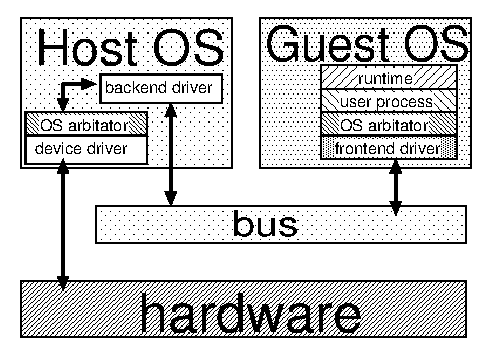
\includegraphics[width=\textwidth]{./xen.eps}
      \caption{既存のハイパーバイザ(ここでは Xen) でのデバイスアクセス}
      \label{existhyp}
    \end{center}
  \end{minipage}
  \begin{minipage}{0.5\hsize}
    \begin{center}
      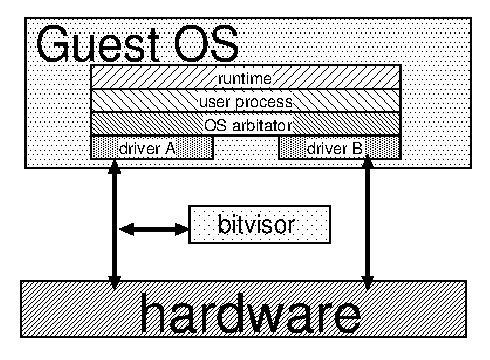
\includegraphics[width=\textwidth]{./bitvisor.eps}
      \caption{parapass-through hypervisor でのデバイスアクセス}
      \label{bitv}
    \end{center}
  \end{minipage}
\end{figure}

それに対し、 Device Masquerading を行う小さなハイパーバイザ ( ここでは Device Masquerading Underlay と呼ぶ ) を導入すると、ゲスト OS ( ここでは Function Kernel と呼ぶ ) には実デバイスの制御を行う必要性がなく図 \ref{underlayarch}、オペレーティングシステムに求められる他の機能の開発に注力できる。 Function Kernel はそれぞれのデバイスクラスに対してただ一つのデバイスドライバさえあればよく、この一つのドライバをすべてのユーザが使ううえ、このドライバは実デバイスを扱わないため、ドライバのカバレッジが高く堅牢になる。%XXX

Device Masquerading Underlay はオペレーティングシステム非依存なため、より多くのユーザが使用でき、より検査されるほか、より多くの開発リソースが期待でき、またそのメリットは複数のオペレーティングシステム開発者に還元されることになる。

\begin{figure}[htbp]
  \begin{minipage}{0.5\hsize}
  \begin{center}
    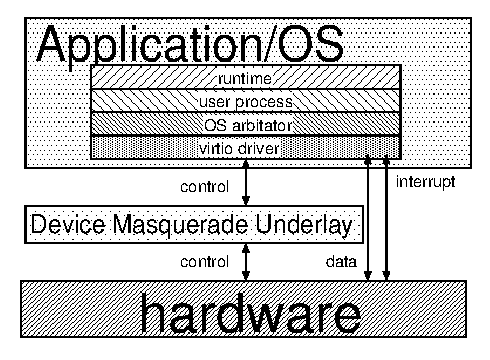
\includegraphics[width=\textwidth]{./underlay.eps}
    \caption{提案手法と伝統的なオペレーティングシステムを組み合わせたデバイスアクセス}
    \label{underlayarch}
  \end{center}
  \end{minipage}
  \begin{minipage}{0.5\hsize}
  \begin{center}
    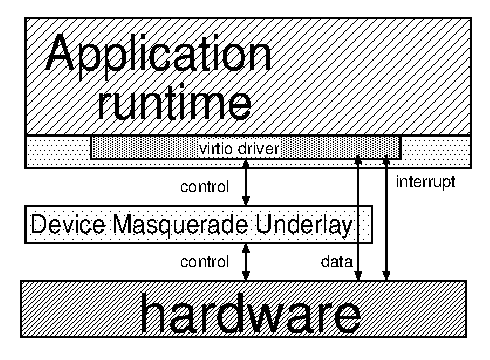
\includegraphics[width=\textwidth]{./underlay_unikernel.eps}
    \caption{提案手法と Unikernel を組み合わせたデバイスアクセス}
    \label{unduni}
  \end{center}
  \end{minipage}
\end{figure}

具体的な実装として、おもに Device Masquerading Underlay は 2つの部分からなる。
第一に、実際のデバイスを制御したり、デバイスとやりとりする部分だ。第二に、virtio デバイスとして振る舞う部分だ。

virtio デバイスとして振る舞う部分は共通のコードを使うことができ、デバイス固有のドライバ部分のみをそれぞれ作成すればよい。この二つのコミュニケーションは Device Masquerading Underlay の内部のバッファを用いて行う。

\begin{figure}[htbp]
  \begin{center}
    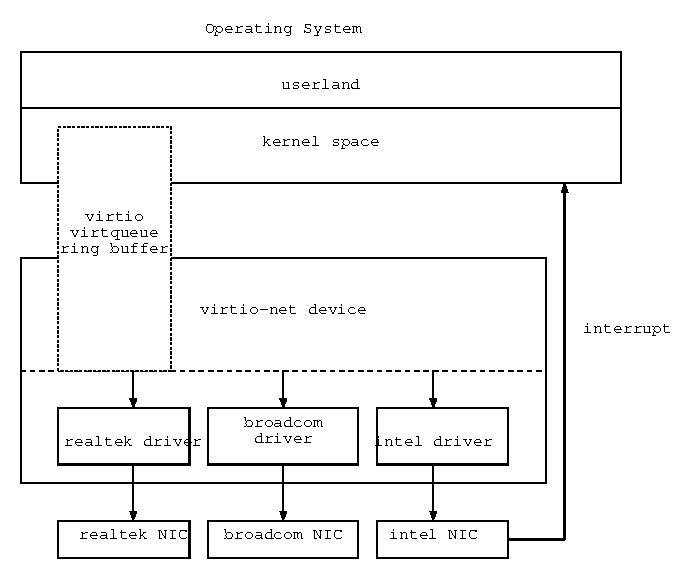
\includegraphics[width=.7\textwidth]{./archtech.eps}
    \caption{Device Underlay Architechture}
    \label{ulayarch}
  \end{center}
\end{figure}


\section{Zero-copy Device Masquerading}

Device Masquerading Underlay は実際のデバイスを制御しつつ、 virtio というデバイスがそこに実在しているかのように見せることで実現とするが、これだけでは性能的な困難が解消できない。そこで本章では、オーバヘッドの解消のための技法を提案する。

まず大きな性能改善の妨げとして、メモリコピーの速度の問題があげられる。オペレーティングシステムは多くの場合、通信の内容を書き込んだメモリの in-kernel buffer をリングバッファとしてデバイスに提供することで高速に通信しているが、図 \ref{underlayarch} のようなアーキテクチャでは、 virtio デバイスとして振る舞う箇所と個別のデバイスドライバの箇所でも同様にバッファを用いてやり取りする。これは不要なコピーが余計に増えていることになる。もっとも遅い箇所は後述のようにデバイスへのコミュニケーションだが、 virtio 化の部分に限るともっとも遅い箇所はメモリコピーであった。

そこでメモリコピーを減らし、不可欠なデバイスへのコピーを除いてメモリコピーを最終的にはゼロにしたい。この手法を独自に Zero-copy Device Masquerading と名付け実装する。図で示すと図 \ref{underlayzerocpy} のようになる。

この技法の概要は、主に Function Kernel から与えられたメモリバッファをそのままデバイスへ書くというものだが、そのためには個別のデバイスドライバが virtio 特有の処理を行わなければならず、図 \ref{underlayarch} で表したような分離が難しくなる。そこで個別のデバイスドライバでの virtio 対応の手間を極力減らすために実装上の工夫が必要となった。

\begin{figure}[htbp]
  \begin{center}
    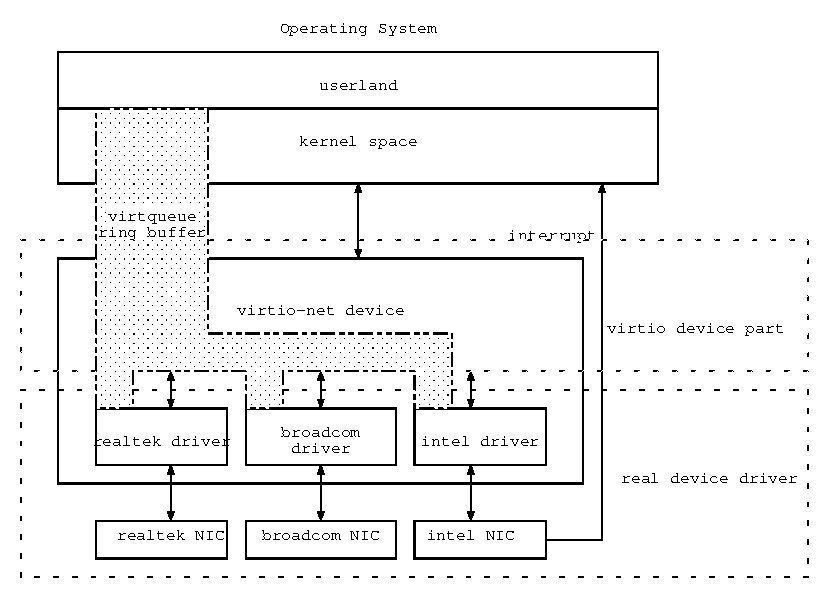
\includegraphics[width=.7\textwidth]{./underlayzerocpy.eps}
    \caption{Zerocopy Device Underlay Architechture}
    \label{underlayzerocpy}
  \end{center}
\end{figure}


%\section{Exitless Device Masquerading}

\chapter{実装}

\section{Device Masquerading Underlay の技術的仕様}

Device Masquerading Underlay の仕様は上記のとおりだが、実装上の制約をいくつか述べる。まず前述のように必須な処理としてOSより先に起動するという点が挙げられる。ここで行う処理は主に、 Device Masquerading Underlay のプログラム領域の保護や、 virtio デバイスの作成、それから virtio 化するターゲットとなるデバイスの検索と初期化だ。

\subsection{Device Masquerading Underlay の隠蔽}

まず自らの隠蔽について述べる。

Function Kernel はどの領域に Device Masquerading Underlay があるのか調べる方法がないので、メモリ領域全体に書き込みを行いかねない。また、自らが管理しているはずのメモリ領域に書いた場合、正しく読み出せなければならない。よって、 Device Masquerading Underlay はそもそも Function Kernel が書き込まず、また万一書いたとしても書いたとおりに正しく読み出せなくてもよい特別な領域を作って「潜む」必要がある。そのような領域として ACPI テーブルの末尾が挙げられる。

ACPI テーブルとは、電源管理やデバイスツリーの管理のために用意されたメモリ領域で、プラットフォームに非依存の標準規格で定められたものだ。 ACPI テーブルはファームウェアによって提供されるが、この領域も Device Masquerading Underlay と同じく上書きされてはならないメモリ領域で、だが Device Masquerading Underlay とは異なり、自らの領域を OS に通達することができる。そこで BitVisor では ACPI テーブルの領域を取得後、その領域に続く場所に自らのプログラムをコピーしなおす。このように起動中の処理として自らのプログラムを再配置する処理は既存のオペレーティングシステムでも一般的な技法だ。しかし BitVisor がこれらとは異なるのは ACPI テーブルの直後の箇所に再配置するという場所の差異の他に、ACPI 領域を取得するオペレーティングシステムの操作をインターセプトして、自らの領域を含めた「より大きい」領域がまるで ACPI テーブル領域として予約されているかのように振る舞うという点となる。このように確保したメモリ領域にオペレーティングシステムが読み書きしようとした場合は無効になり、常に 0 が読み出されるようになっている。このことを可能にするのは SPT または EPT という技術だ。この技術については\ref{aboutEPT}章で解説する。


\begin{figure}[htbp]
\begin{center}
\begin{scaletikzpicturetowidth}{.55\textwidth}
\begin{tikzpicture}[scale=\tikzscale]
\filldraw[fill=green!10!white, draw=green!40!black] (0,0) rectangle (3,10) node[label=above left:640KB]{};
\coordinate (Z) at (3,0);
\draw (0,0) node[label=left:Usable] at (0,3) {} rectangle (3,6) node[label=above right:0x8700]{};
\coordinate (S) at (3,6);
\coordinate (S2) at (13,6);
\draw (0,6) node[label=left:Base Memory Trampoline] at (0,7) {} rectangle (3,8)node[label=above right:0x9700]{};
\coordinate (U) at (3,8);
\coordinate (U2) at (13,8);
\draw (0,8) node[label=left:Device Masquerading Underlay] at (0,9){} rectangle (3,10)node[label=above right:0xffff]{};
\coordinate (H) at (3,10);
\coordinate (H2) at (13,10);
\node at (0.5, -5) {リアルモードでのマッピング};

\filldraw[fill=green!10!white, draw=green!40!black] (20,0) rectangle (23,30) node[label=above left:4GB]{};
\coordinate (B) at (20,0);
\draw (20,27) rectangle (23,28.5);
\coordinate (K) at (20,28.5);
\filldraw[fill=red!20!white, draw=black] (20,8) rectangle (23,10);
\draw (20,4) rectangle (23,10) node[label=right:ACPI テーブル]{};
\coordinate (U3) at (20,10);
\coordinate (S3) at (20,9);
\draw (20,0) rectangle (23,4) node[label=right:DOS互換領域]{};
\draw (20,0) rectangle (23,2.5) node[label=right:レガシー領域]{};
\coordinate (T) at (20,2.5);
\draw [->] (Z)--(B);
\draw [->] (H)--(H2)--(T);
\draw [->] (H)--(H2)--(U3);
\draw [->] (U)--(U2)--(S3);
\draw [->] (U)--(U2)--(K);
\draw [->] (S)--(S2)--(K);
\node at (25, -5) {プロテクトモードでのマッピング};

\end{tikzpicture}
\end{scaletikzpicturetowidth}
\end{center}
\caption{メモリマップ}
\end{figure}

%\begin{tikzpicture}
%\foreach \align [count=\y] in {top, center, base, bottom}{
%    \node at (0,-\y*2) (h1) {host\_entry};
%    \node[BLOCK=4, below=0 of h1,
%    label=left:\align,
%    rectangle split part align=\align]{
%        \nodepart{one}dpid \nodepart{two}port
%        \nodepart{three}IP\nodepart{four}MAC};
%}
%\end{tikzpicture}

Device Masquerading Underlay も BitVisor の技法を踏襲し、 EPT およびメモリマップの構造を取得する命令のインターセプトを用いて Function Kernel からの破壊を防ぎ、セキュリティを担保している。

\subsection{virtio デバイスの実装上の技法}
\label{overview_vio}
一般のハイパーバイザは virtio デバイスをゲストに提供するに当たって新しく作り、 virtio デバイスとして振る舞うエミュレータがアプリケーションとして動作するため、それぞれのハイパーバイザが動作するオペレーティングシステムでのネットワーク通信用のブリッジなどと通信すればよい。しかし本論文での実装では、一つの実在するハードウェアに相当する virtio デバイスを作成し関連付けるので、より効率的な作成方法が考えられる。

この方法を順を追って説明する。

\begin{enumerate}
\item 後述のように Masquerading の対象となるデバイスを発見する
\item その PCI configuration 空間に virtio の PCI configuration 空間として有効なものとなるようフック関数を用意する (PCI configuration 空間については\ref{about_pciconfig}章で後述する)
\item Function Kernel は Base Address Register (BAR) と呼ばれる領域のビットマスクを最初に読み出すので適切な値をフック関数で返す
\item のちにそれぞれのデバイスに相当するデバイスドライバを割り振るために Vendor ID と Device ID を読み出す必要があるので、これを virtio のものにする
\item Function Kernel はそれぞれのデバイスに相当するドライバが確定すると、その固有のドライバをアサインするので virtio の規格に則り各フィールドを適切な値として返す
\end{enumerate}

これによって、新たにデバイスの領域を作りだすかわりに、デバイスの種類をすり替えることが出来るようになる。このことで、実際のデバイスが存在するバスの位置に virtio デバイスが存在するように見せかけられるので、抽象化の行き過ぎによる混乱をさけることが出来る。また、新たにデバイスを作成するには PCI configuration 空間を発見するための ACPI テーブルごと変える必要があるが、これは専用の中間言語で操作される高度に複雑なもので、このことでコードサイズが無用に大きくなってしまい attack surface が拡大するが、このすげ替えによる virtio デバイスの作成によって簡単に実際のデバイスの隠蔽も出来、コードサイズ小さくなって処理が簡単になるため、よりよい。

\subsection{適切なデバイスドライバの検索とハンドリング関数への関連付け}

デバイスの探索には ACPI テーブルを読み出して PCI configuration 空間を発見し、ターゲットとなるデバイスを示す ID を持っているものを見つけなければならない。適切な ID とそれに合った初期化ルーチンの関連付けは \lstinline!struct pci_driver! と呼ばれる構造体として記述し、この構造体をリストに登録する上位の初期化ルーチン\lstinline!void pci_register_driver(struct pci_register)!を用いて登録する。この上位の初期化ルーチンは、前述したデバイス固有の初期化ルーチンとは異なって、実在するデバイスの数のみならず対応しているデバイスのドライバの数だけ呼び出される必要があるが、小さな linked list への登録をそれぞれ一度だけ行うものなのでこの実行のコストは無視できる。

\lstinline!void pci_register_driver(struct pci_driver *)!を実行する関数は \lstinline!PCI_DRIVER_INIT(X)!と呼ばれるマクロを通して登録される。 BitVisor ではいくつかの\lstinline!_INIT!で終わる名前のマクロが存在し、ここで与えられた関数は、このマクロの優先度の順に実行される。\lstinline!PCI_DRIVER_INIT!マクロは PCI デバイスの初期化よりも前に実行され、ここで呼ばれた\lstinline!void pci_register_driver(struct pci_driver *)!によって登録された\lstinline!struct pci_driver!型のグローバル変数は ACPI テーブルを BitVisor が解釈した際に探索され、この構造体のメンバ関数である\lstinline!.new!が呼ばれるためにある。このメンバ関数として与えられた初期化ルーチンには、引数としてデバイスオプションが与えられ、このオプションはデバイスの種別やバスの位置などに基づいてユーザがオプションとして与えるものだ。

ここでマッチした構造体のメンバ関数は、与えられたオプションや PCI デバイスの固有の情報を与える\lstinline!struct pci_device!という構造体を用いて初期化を行い、上述のような処理を行うフック関数などを登録して終了する。

理解のためにソースコードの一部分を示す。

\begin{lstlisting}
static void
bnx_new (struct pci_device *pci_device)
{
  :
  :
  :
}

static struct pci_driver bnx_driver = {
	.name		= driver_name,
	.longname	= driver_longname,
	.driver_options	= "tty,net,virtio",
	.device		= "class_code=020000,id="
			  "14e4:165f|" /* BCM5720 */
			  "14e4:165a|" /* BCM5722 */
			  "14e4:1682|" /* Thunderbolt - BCM57762 */
			  "14e4:1684|" /* BCM5764M */
			  "14e4:1686|" /* BCM57766 */
			  "14e4:1691|" /* BCM57788 */
			  "14e4:16b4", /* BCM57765 */
	.new		= bnx_new,
	.config_read	= bnx_config_read,
	.config_write	= bnx_config_write,
};

static void
bnx_init (void)
{
	pci_register_driver (&bnx_driver);
}

PCI_DRIVER_INIT (bnx_init);
\end{lstlisting}

ここで、\lstinline!PCI_DRIVER_INIT!マクロによって\lstinline!void bnx_init(void)!が呼ばれることが約束される。これが呼ばれると \lstinline{struct pci_driver bnx_driver} が登録される。もし BitVisor が起動時にこの構造体の \lstinline{.device} で示される文字列に相当する Vendor ID 及びデバイス ID のいずれかを持っている PCI デバイスを発見した場合は、その場で \lstinline{.new} で示された \lstinline{void bnx_new (struct pci_device *pci_device)} を呼ぶ。この中でデバイスを初期化したり、前述のフック関数を登録したりするということになる。


\section{EPTによるフックの動作}
\label{aboutEPT}
EPT とは、 Extended Page Table の略称で、 Second Level Address Translation という技術の Intel 製品での実装を指す。まず読者のために、ページテーブルについて軽く説明する。

近代的なアプリケーションは実際のメモリの上で直接動作する代わりに、固有のメモリアドレス空間の上で動作している。しかし固有のメモリ空間を作り出しつつ実際に動作するためには、そのアドレス空間と実際のメモリ空間との間を関連付ける方法が必要になる。その一つとしてセグメント方式が挙げられる。しかし、より高度な分離を行う必要が出てきたのでその後実装された変換方式がページテーブルだ。

ページテーブルは 32bit あるいは 64bit のアドレスを、下位の 12bit と残りの 10bit ずつのキーに分割する。それぞれのキーのうちもっとも上位のものをインデックスとしてアドレス変換テーブルを引き、それで得たテーブルに対し残りの最も上位のキーをインデックスとして用いてさらに引き、引き終わったものに先ほどの 12bit を append してアドレスを得る。

この場合最初に引くテーブルをプロセスごとにあてがえば、プロセスごとに独立した空間を作ることができるため良いアドレス変換が出来る。この最初に引くテーブルを指定するものがCR3レジスタと言われる特殊なレジスタだ。

現在使われているオペレーティングシステムのほぼすべてはこの仕組みを利用してアドレス変換を行ってプロセスを独立させている。

\begin{figure}[htbp]
  \begin{center}
\begin{scaletikzpicturetowidth}{.9\textwidth}
\begin{tikzpicture}[scale=\tikzscale, every node/.append style={draw}]
  \node (mem)
        [rectangle split, rectangle split horizontal,
         rectangle split parts=3, text width=16ex, text height=2ex, centered,
         rectangle split part align=center
        ]
        {\nodepart{one} \raisebox{1pt}{10bit}\strut
         \nodepart{two} 10bit\strut
         \nodepart{three} 12bit\strut
        };

  \node (table1)
            [rectangle split, rectangle split parts=10, draw, below right=of mem.one] 
     {  \nodepart{one} \textbf{Pagetable}
       \nodepart{six} \footnotesize{該当するエントリ}
    };
  \node (table2)
            [rectangle split, rectangle split parts=10, draw, below right=of mem.two] 
     {  \nodepart{one} \textbf{Pagetable}
       \nodepart{two} \footnotesize{該当するエントリ}
    };
  %\node (table3)
  %          [rectangle split, rectangle split parts=10, draw, below=of mem.three] 
  %   {  \nodepart{one} \textbf{Pagetable}
  %     \nodepart{four}
  %  };
   \node (CR3) at (-30, -10) [rectangle] {CR3レジスタ};
   \node (add) at (20, -10) [circle] {+};
   \coordinate (pm) at (35, -10);

  \draw[-{Stealth[scale=1.3,angle'=45]}] (mem.one south) -- (table1.one north);
  \draw[-{Stealth[scale=1.3,angle'=45]}] (mem.two south) -- (table2.one north);
  %\draw[-{Stealth[scale=1.3,angle'=45]}] (mem.three south) -- (table3.one north);
  \draw[-{Stealth[scale=1.3,angle'=45]}] (table1.six east) -- (table2.one west);
  \draw[-{Stealth[scale=1.3,angle'=45]}] (table2.two east) -- (add);
  %\draw[-{Stealth[scale=1.3,angle'=45]}] (table3.four east) -- (add);
  \draw[-{Stealth[scale=1.3,angle'=45]}] (mem.three south) -- (add);
  \draw[-{Stealth[scale=1.3,angle'=45]}] (add) -- (pm);
  \draw[-{Stealth[scale=1.3,angle'=45]}] (CR3) -- (table1.one west);
\end{tikzpicture}
\end{scaletikzpicturetowidth}
  \caption{ページディレクトリ方式のページテーブルでのアドレス変換の概略図}
  \end{center}
\end{figure}

このようなアドレス変換のおもな目的として、プロセス空間の分離やセキュリティが挙げられる。プロセスのアドレス空間と物理的なメモリ空間を別のものとして扱うことで、プラットフォーム全体へのアクセスを限定することができる。例えば、リングプロテクションと併用することで、プロセスは CR3 を書き換えられず、プロセス同士の侵入やプラットフォームへの直接のアクセスを防ぐことが出来る。

同様の仕組みを仮想化支援機構として導入したのが、 Second Level Address Translation だ。この仕組みは、上に挙げたようなアドレス変換を一段目とし、そこで得たアドレスをさらに変換するというものだ。


\begin{figure}[htbp]
  \begin{center}
		%\includegraphics[width=0.8\textwidth]{ept.tikz}
		\resizebox{\textwidth}{!}{
		\begin{tikzpicture}[every node/.append style={draw}]
  \node (mem)
        [rectangle split, rectangle split horizontal,
         rectangle split parts=3, text width=16ex, text height=1ex, centered,
         rectangle split part align=center
        ]
        {\nodepart{one} \raisebox{1pt}{10bit}\strut
         \nodepart{two} 10bit\strut
         \nodepart{three} 12bit\strut
        };
  \node (table1)
            [rectangle split, rectangle split parts=10, draw, below right=of mem.one] 
     {  \nodepart{one} \textbf{Pagetable}
       \nodepart{six} \footnotesize{該当するエントリ}
    };
  \node (table2)
            [rectangle split, rectangle split parts=10, draw, below right=of mem.two] 
     {  \nodepart{one} \textbf{Pagetable}
       \nodepart{two} \footnotesize{該当するエントリ}
    };
   \node (CR3) [rectangle, left=8mm of table1] {CR3レジスタ};
   \node (add) [circle, right=8mm of table2] {+};
   \coordinate (pm) at (16, -5);
  \node (pmm)
        [rectangle split, rectangle split horizontal,
         rectangle split parts=3, text width=16ex, text height=1ex, centered,
         rectangle split part align=center, right=3mm of add
        ]
        {\nodepart{one} \raisebox{1pt}{10bit}\strut
         \nodepart{two} 10bit\strut
         \nodepart{three} 12bit\strut
        };

  \node (table3)
            [rectangle split, rectangle split parts=10, draw, below right=of pmm.one] 
     {  \nodepart{one} \textbf{EPT}
       \nodepart{four}\footnotesize{該当するエントリ}
    };
  \node (table4)
            [rectangle split, rectangle split parts=10, draw, below right=of pmm.two] 
     {  \nodepart{one} \textbf{EPT}
       \nodepart{seven}\footnotesize{該当するエントリ}
    };
   \node (EPTP) [rectangle, left=8mm of table3] {EPTP};
   \node (add2) [circle, right=8mm of table4] {+};
  \draw[-{Stealth[scale=1.3,angle'=45]}] (mem.one south) -- (table1.one north);
  \draw[-{Stealth[scale=1.3,angle'=45]}] (mem.two south) -- (table2.one north);
  %\draw[-{Stealth[scale=1.3,angle'=45]}] (mem.three south) -- (table3.one north);
  \draw[-{Stealth[scale=1.3,angle'=45]}] (table1.six east) -- (table2.one west);
  \draw[-{Stealth[scale=1.3,angle'=45]}] (table2.two east) -- (add);
  %\draw[-{Stealth[scale=1.3,angle'=45]}] (table3.four east) -- (add);
  \draw[-{Stealth[scale=1.3,angle'=45]}] (mem.three south) -- (add);
  \draw[-{Stealth[scale=1.3,angle'=45]}] (add) -- (pmm);
  \draw[-{Stealth[scale=1.3,angle'=45]}] (CR3) -- (table1.one west);
  \draw[-{Stealth[scale=1.3,angle'=45]}] (EPTP) -- (table3.one west);
  \draw[-{Stealth[scale=1.3,angle'=45]}] (pmm.one south) -- (table3.one north);
  \draw[-{Stealth[scale=1.3,angle'=45]}] (pmm.two south) -- (table4.one north);
  \draw[-{Stealth[scale=1.3,angle'=45]}] (table3.four east) -- (table4.one west);
  \draw[-{Stealth[scale=1.3,angle'=45]}] (table4.seven east) -- (add2);
  \draw[-{Stealth[scale=1.3,angle'=45]}] (add2) -- (pm);
  \draw[-{Stealth[scale=1.3,angle'=45]}] (pmm.three south) -- (add2);
\end{tikzpicture}

	}
  \end{center}
  \caption{ページテーブルとEPTを組み合わせたアドレス変換の概略図}
\end{figure}

これを行うことで、仮想化ゲストのオペレーティングシステムはハイパーバイザを配慮してメモリを配置したり、あるいはハイパーバイザがゲストのオペレーティングシステムの CR3 を監視して、プロセスが代わるたびに CR3 をセットしたりする必要がなくなった。

ゲストは一般のハードウェアの上で動作しているという前提でアドレス空間を利用してよいし、またそのアドレス空間が物理的にどこにマップされるかはハイパーバイザが決定することが出来るようになった。

Intel の仮想化支援機構では、 VMCS と呼ばれる仮想化ゲストが発行出来る命令やその他の様々な制御用構造体が用意されていて、これをセットアップすることで仮想マシンを作ることが出来る。 EPT によるアドレス変換の際のエラーハンドリングや、 IO 命令発行時のハンドリングなどをする際には、それらが終了理由になるようにし、 \texttt{vmlaunch} 及び \texttt{vmresume} 命令により、セットアップした VMCS を実際にゲストとして実行してからそのコンテキストが終了するまで待つと、こうしたイベントをフック出来るようになる。

EPT やページテーブルのエントリには、次のテーブル(ディレクトリ)へのポインタの他に制御用のビットフィールドがあり、これによってページのサイズやエラー時に起きるべき例外の選択などが出来る。

\section{virtio の仕様について}

virtio は準仮想化デバイスのデファクトスタンダードとして広く用いられており、ライブラリ OS のライブラリでもサポートされる数少ないデバイスだ。この仕様は一度大きく変わっている。今回は既に普及している古い規格ではなく、性能改善のため新しい virtio 1.0 と呼ばれる規格に準拠する。以降の説明は virtio 1.0\cite{virtio_spec} での定義にしたがう。

この規格では、デバイスをその動作の種別によっていくつかのデバイスクラスに分けている。最もよく知られたものに virtio-net と呼ばれるネットワーククラスがある。今回はこれを proof-of-concept の実装として対象にした。このクラスは最もよく知られ、広く利用されているだけでなく、パフォーマンスの測定に便利だという特徴がある。この他のデバイスクラスとして、コンソールやブロックデバイス、ビデオカードなどが挙げられる。

デバイスは起動時の検索によって発見されなければならないが、 virtio 自身はその方法を定めていない。 virtio デバイスは、以下の 3 つのバス規格のうち 1 つを利用することになっている。

\begin{itemize}
\item PCI
\item MMIO
\item Channel-IO
\end{itemize}

このうち、 Channel-IO は IBM の専用のハードウェアを前提にしたもので、今回は実装の対象ではない。また、 MMIO の場合はそもそもバスというよりは PCI のようなデバイス検索の機能を持つハードウェアを利用できない組み込みプラットフォームなどを対象にしたもので、 MMIO 空間のどこにマップされるか予め管理者が入力しておくというものだ。これは不便で、 PCI が使える場合には使われず、あまり知られていないので今回は実装の対象としない。

今回は PCI バスでドライブされる virtio デバイスを作成することとした。これは最もよく知られた規格で、 ACPI によって PCI バスは列挙されているのでデバイス検索が可能であり、 Function Kernel の可移植性を引き上げることが出来る。

一般にこの場合 virtio デバイスとして振る舞う PCI configuration 空間を作成する必要があるが、本研究で提案するアーキテクチャの場合、新たにデバイスを作り出すのではなく既存のデバイスを Function Kernel からみて virtio デバイスとして振る舞わせ、利用させるので、既存のデバイスの PCI コンフィギュレーション空間を活用すれば良い。

\subsection{PCI configuration 空間について}
\label{about_pciconfig}

このサブセクションでは、デバイスを使うゲスト上のソフトウェアをドライバ、 virtio デバイスを含む PCI デバイスをデバイスと呼ぶ。

PCI configuration 空間とは、 PCI デバイス固有のアドレス空間で、 0x00 番地から 0xff 番地までが利用できる。このうち特に 0x00 番地から 0x3f 番地まではそれぞれのフィールドの意味が決まっている。

ここで、特に説明に必要なフィールドについて先に列挙する。

\begin{itemize}
\item Vendor ID
\item Device ID
\item BAR[0..5]
\item Subsystem Vendor ID
\item Subsystem ID
\item Capability pointer
\end{itemize}

ここで、 BAR とは、\ref{overview_vio}章ですでに触れた BAR のことだ。 VendorID と Device ID は適切なデバイスドライバを発見するために必要なもので、デバイスの製品ごとに固有のものだ。これについてもすでに触れた。Subsystem Vendor ID や Subsystem ID も Vendor ID や Device ID と同じ機能を持つ。

Capability とは、 PCI configuration 空間で予め定められたフィールド以外の設定をデバイスが通知したい時に、 PCI configuration 空間内に linked list を作ることになっているが、そのリストの head を指す番地が入るのが Capability pointer だ。

BAR はドライバとデバイス双方が読み書きする32bitの領域だ。ここでアドレスなどがやり取りされることが多い。 BAR について、ここにかかれた値が具体的に何に使われるのかは定められていないが、メモリ上のなんらかの構造体へのポインタをやり取りして、その構造体を用いてデバイスとドライバがコミュニケーションすることが多い。 virtio も同様に BAR に virtio 固有の設定をするための構造体を示すアドレスがドライバからかかれることになっている。このような使い方をする際、単純にどのようなアドレスがデバイスに支給されても必ず使えるとは限らない。 PCI はプラットフォームに非依存の規格であるから、例えばバイトアドレッシングに対応していないデバイスで、下位 2bit が 00 でなければ動作しないデバイスや、キャッシュを跨いでいると使えないデバイス、あるいは DMA の都合上一定のアドレス領域でなければならないということがありえる。このような場合に備え、 BAR へ書くことができるアドレスを調べる方法が用意されている。 BAR に書けないビットは何を書いても同じ内容しか読み出せないはずだ。ということは、まず全ビットを 0 にして書き込み、読み出してからまた全ビットを 1 にして書き込んで読み出して比べると、書き込めるビットが分かる。

また、 BAR の下位 2bit あるいは 4bit には意味がある。下位 1 bit
(\tikz{ \draw (0,0) rectangle (3.2,1.3ex); \filldraw[fill=red!40!black, draw=black] (3.1,0) rectangle (3.2, 1.3ex); \node at (3.15, 2ex){\small{1}}})
が 1 であった場合、その BAR にかかれた値は PIO 空間へのポインタとなる。その場合、 2 bit
(\tikz{ \draw (0,0) rectangle (3.2,1.3ex); \filldraw[fill=red!40!black, draw=black] (3,0) rectangle (3.1, 1.3ex); \node at (3.05, 2ex){\tiny{\times}}})
めは予約領域だ。下位 1bit
(\tikz{ \draw (0,0) rectangle (3.2,1.3ex); \filldraw[fill=red!40!black, draw=black] (3.1,0) rectangle (3.2, 1.3ex); \node at (3.15, 2ex){\small{0}}})
が 0 であった場合、その BAR にかかれた値はメモリ空間へのポインタとなる。その場合、そこから数えて上位 2bit
(\tikz{ \draw (0,0) rectangle (3.2,1.3ex); \filldraw[fill=red!40!black, draw=black] (2.8,0) rectangle (3.1, 1.3ex); \node at (2.95, 2ex) {\small{??}} })
はアドレスの大きさを指し、その次のビット
(\tikz{ \draw (0,0) rectangle (3.2,1.3ex); \filldraw[fill=red!40!black, draw=black] (2.7,0) rectangle (2.8, 1.3ex); \node at (2.75, 2ex) {\small{?}}})
はプリフェッチ可能か示すビットだ。

ここで指定されたアドレスには、一体どのような構造体がくるのだろうか。実は virtio では、ここで交換すべき情報として 5 つの構造体が定義されている。 BAR には 6 つのエントリがあるが、これを対応させるのは capability list で行う。

\subsection{virtio の capability list について}

これら 5 つの構造体の種別と BAR 番号をひもづける capability list の構造は virtio の規格で決まっている。

そもそも capability list とは以下のようなもので、特にその capability のエレメントがどのような意味をもつのかを表す \texttt{ID} と 次のエレメントへのポインタはどの capability であっても必ず書いてあり、それぞれのオフセットは 0 と 1 だ。リストの最後の要素は、次のエレメントへのポインタとして 0 と書いてなければならない。

\begin{figure}[htbp]
  \begin{center}
\begin{scaletikzpicturetowidth}{.9\textwidth}
\begin{tikzpicture}[scale=\tikzscale, ->, >=stealth', every node/.append style={draw}]
  \node (cfg)
            [rectangle split, rectangle split parts=10, draw]
     {  \nodepart{one} \textbf{PCI configuration 空間}
       \nodepart{four} \footnotesize{:}
       \nodepart{five} \footnotesize{:}
       \nodepart{six} \footnotesize{Capability ptr}
    };
  \node (cap1) 
            [rectangle split, rectangle split parts=8, draw, right=2 of cfg]
            {\nodepart{one} \hypertarget{cap1}{\textbf{Capability エレメント}}
       \nodepart{two} \footnotesize{ID}
       \nodepart{three} \footnotesize{次のエレメントへのポインタ}
       \nodepart{four} \footnotesize{長さ}
       \nodepart{five} \footnotesize{種別}
       \nodepart{six} \footnotesize{BAR 番号}
       \nodepart{seven} \footnotesize{オフセット}
       \nodepart{eight} \footnotesize{構造体の長さ}
    };
  \node (cap2)
            [rectangle split, rectangle split parts=6, draw, below=3 of cap1] 
     {  \nodepart{one} \textbf{Capability エレメント}
       \nodepart{two} \footnotesize{ID}
       \nodepart{three} \footnotesize{次のエレメントへのポインタ}
       \nodepart{four} \footnotesize{:}
    };
  \node (cap3)
            [rectangle split, rectangle split parts=6, draw, left=2 of cap2] 
     {  \nodepart{one} \textbf{Capability エレメント}
       \nodepart{two} \footnotesize{ID}
       \nodepart{three} \footnotesize{次のエレメントへのポインタ}
       \nodepart{four} \footnotesize{:}
    };
   \node (zero) [draw, circle, left=1 of cap3] {0};
  \path[every node/.style={font=\sffamily\small}]
    (cfg.six east) edge[bend left] node [right] {} (cap1.one west)
  (cap1.three east) edge[bend left] node [right] {} (cap2.one east)
  (cap2.three west) edge[bend right] node [right] {} (cap3.one east)
  (cap3.three west) edge node [right] {} (zero)
  ;
\end{tikzpicture}
\end{scaletikzpicturetowidth}
  \caption{Capability list}
  \end{center}
\end{figure}

ここで、\hyperlink{cap1}{最初の capability エレメント}は、 virtio の capability list の形をしている。長さはこのエレメントの長さ、種別は構造体の種別を表している。

実際にこのような capability list を作るのは簡単で、このリストも PCI configuration 空間内のものだから、 PCI configuration 空間と同様に改変すれば良い。

ただし、このエレメントはどの内容だろうと自在に配置されてしまうので、 MSI 割り込みを有効にする場合には困難が伴う。というのは、 MSI 割り込みの capability list は MSI 割り込みを利用する場合には必須だが、このフィールドの内容はデバイスの実際の内容を反映しなければならないし、ドライバが提供するアドレス情報やデータ情報をデバイスに書き戻さなければならない。こうした情報を BitVisor で予め読み書きし、ドライバから書き込まれた場合にはその内容を書き戻す必要がある。これは、デバイスに提供した MSI 割り込みの capability list の位置とは異なる可能性があるうえ、このエレメントに示される``次のエレメントへのポインタ''は無効な値であるから適宜読み替えなければならない。さらにその上、こうした capability list の要素が多いデバイスは、 PCI configuration 空間とはアクセスの方法が全く異なる Extended PCI configuration 空間にも情報が書いてある可能性があるので、 MSI 割り込みを必ず有効にするということは大変だ。

\subsection{PCI configuration 空間の改変}

PCI configuration 空間の改変には、Function Kernel からの PCI configuration 空間の読み書きをインターセプトして改変すれば良い。 PCI configuration 空間への読み書きは \texttt{in/out} 命令で行うので、上記の方法でフックすれば良いことになる。起動時に読み書きするだけで、その後頻繁に読み書きするものではないから、多少のオーバヘッドは性能に一切影響を与えない。このことはのちのベンチマークで明らかになる。

PCI configuration 空間への読み書きのインターセプトは既に先行の実装\cite{bitvisor}で提供される仕組みを用いると簡単に実装できる。しかし、 BitVisor の多くの実装では、今回のようにたくさんのフィールドを改変するわけではないため、そのままこの仕組みを利用すると煩雑になってしまう。そこである程度宣言的に書けるよう工夫をした。

\section{virtqueue の仕様について}

virtqueue とは、 virtio の仕様の根幹をなす機能だ。これはメモリのリングバッファになっていて、 virtio を用いた Function Kernel と Device Masquerading Underlay の通信の多くはこのリングバッファを経由して行う。 virtqueue のメモリはドライバの責任で用意する。デバイスはゲストが用意したメモリを読み書きし、使い終わったら返却する。この仕組みを利用して\tikz[baseline=-0.5ex]{\node(v){デバイス};\node(r)[right=1cm of v]{ドライバ};\draw[<->] (v) -- (r);}間の読み書きを行う。

virtqueue のリングバッファのエレメントは任意の大きさのバッファだ。このバッファのライフサイクルを示す。

\begin{figure}[H]
  \begin{center}
\begin{scaletikzpicturetowidth}{.9\textwidth}
\begin{tikzpicture}[scale=\tikzscale, ->, >=stealth']
  \node (u) [circle, fill=koke, draw]{Uninitialized};
  \node (i) [circle, fill=usugaki, draw, right=7 of u] {initialized};
  \node (k) [circle, fill=seji, draw, below=of i] {Available};
  \node (t) [circle, fill=kincha, draw, left=7 of k]  {Used};
  \draw[->] (u) edge node[auto]{\small{Function Kernel がこのバッファの情報を登録する}} (i)
            (i) edge node[left]{\small{Function Kernel がバッファを Available にする}}(k)
            (k) edge node[auto]{\small{Device Masquerading Underlay がバッファを使う}}(t)
            (t) edge node[auto]{\small{Function Kernel が取り出す}}(u);
\end{tikzpicture}
\end{scaletikzpicturetowidth}
  \caption{virtqueue の 1 バッファのライフサイクル}
  \end{center}
\end{figure}

また、これらのバッファを複数管理するためにリングバッファになっているので、そのリングバッファの構造を示す。
リングバッファは、\texttt{used}と\texttt{avail}と呼ばれるカウンタによってその一部を指されている。\texttt{avail}が\texttt{used}に追い抜かれないという制約を付けると、必ずデバイスにとって available なバッファは $ used \leq x < avail $ の間にあるということが分かる。さらに、リングバッファに直接データを書くのではなく、リングバッファがデータをやり取りする場所を指し示すようにすることで、リングバッファ全体の大きさを一定に保つほうが良い。

\begin{figure}[H]
  \begin{center}
\begin{scaletikzpicturetowidth}{.9\textwidth}
\begin{tikzpicture}[scale=\tikzscale, ->, >=stealth']
  \node (avail) [rectangle, draw] {avail};
  \node (used) [rectangle, draw, right of=avail] {used};
  \foreach \x in {0,...,9} {
    \ifthenelse{\x=4 \OR \x=5}{\def\mycolor{red!15}}{\def\mycolor{blue!14}}
    \node (b\x) at (-\x*360/10+90:3) [fill=\mycolor,draw, circle]{buffer\x};
    \coordinate (p\x) at (-\x*360/10+90:5);
    \draw[->] (b\x) -- (p\x);
    }
  \foreach \x/\y in {0/1, 1/2, 2/3, 3/4, 4/5, 5/6, 6/7, 7/8, 8/9, 9/0} {
    \draw[->] (b\x) to [bend left] (b\y);
  }
  \draw[->] (avail) -- (b6);
  \draw[->] (used) -- (b4);
  \node (upage) at (p2) [draw, fill=byakuroku, rectangle, minimum width=5ex, minimum height=10ex, align=center] {used\\ page};
  \node (upage2) at (p3) [draw,fill=byakuroku, rectangle, minimum width=5ex, minimum height=13ex, align=center] {used\\ page};
  \node (page) at (p4) [draw, fill=yamabuki!50, rectangle, minimum width=5ex, minimum height=10ex] {page};
  \node (page2) at (p5) [draw,fill=yamabuki!50, rectangle, minimum width=5ex, minimum height=13ex] {page};
  \node (page3) [draw, fill=gray!50, rectangle, minimum width=5ex, minimum height=13ex, below left=0.4 of page2] {page};
  \node (page4) [draw,fill=gray!50, rectangle, minimum width=5ex, minimum height=13ex,  left=0.4 of page3] {page};
  \node (page5) [draw,fill=gray!50, rectangle, minimum width=5ex, minimum height=13ex,  left=0.4 of page4] {page};
  \node (page6) [draw,fill=gray!50, rectangle, minimum width=5ex, minimum height=13ex,  left=0.4 of page5] {page};
  \draw[->] (b5) -- (page2);
  \draw[->] (b4) -- (page);
\end{tikzpicture}
\end{scaletikzpicturetowidth}
  \caption{リングバッファの構造}
  \end{center}
\end{figure}

このリングバッファを作るために必要なデータについて考えると、\texttt{avail} と \texttt{used} のポインタだけでなく、データをやり取りする \texttt{page} の状態や隣のリングバッファの番号などを保持する各リングバッファの要素のディスクリプタを作った方が良い。実際 virtqueue はこの通りに作られている。

virtqueue を構成する具体的な要素について列挙する。

\begin{itemize}
  \item ディスクリプタ
  \item Available Ring
  \item Used Ring
\end{itemize}

以上のエントリが連続しているメモリ領域を Function Kernel が作成し、 PCI 経由で通達した構造体を通して Device Masquerading Underlay に通達する。このメモリ領域の定義の抜粋を示す。

\begin{lstlisting}[language=C]
struct virtq_desc {
/* Address (guest-physical). */
le64 addr;
/* Length. */
le32 len;
/* This marks a buffer as continuing via the next field. */
#define VIRTQ_DESC_F_NEXT 1
/* This marks a buffer as device write-only (otherwise device read-only). */
#define VIRTQ_DESC_F_WRITE 2
/* This means the buffer contains a list of buffer descriptors. */
#define VIRTQ_DESC_F_INDIRECT 4
/* The flags as indicated above. */
le16 flags;
/* Next field if flags & NEXT */
le16 next;
};
\end{lstlisting}

\texttt{virtq\_desc} は、個々のバッファで、図のように linked list になっている。それぞれ Function Kernel から見たバッファのアドレスが書いてあり、また有効な長さが書いてある構造体だ。\texttt{virtq\_avail} は、 \texttt{avail}状態のバッファの先端の次を指しているほか、いくつかの情報を持っている。 \texttt{virtq\_used} は \texttt{used} 状態のバッファの次を指している。

なぜそれぞれ次のバッファを指しているかというと、もし使用済のデータを指すようであれば、初期化時の値が不明になってしまうからだ。次くる場所を指すようにすれば、当然 0 番目からスタートするので間違いがなくてすむ。

\section{virtio-net の仕様について}

virtio-net とは、 virtio の標準規格\cite{virtio_spec}で定められたデバイスクラスのひとつで、ネットワーク機能を提供する。virtio-net のデバイスは 3 つのキューを持つ。それぞれ、送信キュー、受信キュー、コントロールキューと呼ぶ。

ここでやり取りされるデータには 12 バイトのヘッダがついていて、その後にはネットワークのイーサネットフレームが続く。また、フレームが一つのバッファに入りきらないことがありえる。そのような場合は後続のデータに続いている。後続のデータは、リングバッファで示された次の要素が指し示している。 Linux のドライバはヘッダとフレームを別々に送ることが多いが、特に仕様で決まっているわけではない。

\subsection{送信時の動作}

送信キューは、 Function Kernel が外にデータを送りたいときに用いられ、 Function Kernel がそこに書き終わると DeviDevice Masquerading Underlay に通知する。 Device Masquerading Underlay はそこから取り出して実際のデバイスに割り振って送信する。

送信すべき内容は Function Kernel がまず Avail リングバッファに格納し、 avail インデックスを進める。デバイスには notification 構造体へ書き込みのアクセスが行われ、このタイミングでメモリアクセスをフックし Device Masquerading Underlay が avail インデックスと used インデックスを比較、間にあるバッファを送信する。

データを送信し終わると Device Masquerading Underlay は used インデックスを進める。

Used リングバッファに格納された使用済ページは Function Kernel によって破棄される。

\subsection{受信時の動作}

受信キューは、 実デバイスが Function Kernel に割り込みを通達すると、 Function Kernel が Device Masquerading Underlay の割り込み原因レジスタを見にくるので、そのタイミングで実デバイスから Device Masquerading Underlay が情報を取り出し、 Function Kernel に処理を戻す。

あらかじめ Function Kernel は多めに空白ページを確保しておき、 avail リングバッファにつないでおく。 Device Masquerading Underlay が受信処理をし、書き込み終わったものから順番に used リングバッファにつなぎ、 used インデックスを進める。このとき、 Function Kernel は割り込みを受けて原因レジスタを見にきたところなので、ここでパケットの受信による割り込みであると通達することでこの used リングバッファを Function Kernel が消費して受信処理が完了する。消費し終わったページはやはり Function Kernel が破棄する。適宜のタイミングで Function Kernel は avail リングバッファを補充する。この補充が遅れるとネットワーク性能に影響がでてしまう。

%\subsection{制御}
%\section{Exitless Device Masquerading の仕組み}

\chapter{評価}

\section{実験環境について}

\subsection{ハードウェア}
今回の計測では、 Panasonic 社製 Let's note CF-AX3 を用いた。

\begin{description}
\item[CPU] Core i7 4500U @ 1.8GHz
\item[メモリ] DDR3 4GB
\item[ネットワークチップ] I218-M
\end{description}

\subsection{コンパイラ}

今回計測に用いた実行形式のデータのうち、 Device Masquerading Underlay は gcc (GCC) 5.3.0 で生成し、 Function Kernel として用いた Linux は gcc (Ubuntu 5.2.1-22ubuntu2) 5.2.1 で生成した。

\subsection{Function Kernel}

今回計測に用いた Function Kernel には、 linux 4.4.0-rc3 を用いた。

\section{実験の概要}

今回実装した \tikz[baseline=-0.5ex]{\node(v){virtio};\node(r)[right=1cm of v]{実デバイス};\draw[<->] (v) -- (r);} 変換の性能を評価するため、ネットワークの速度評価で知られる netperf と ping で実験を行った。

また、本研究での実装で、性能に影響を与える可能性があるパラメータとしてキューのサイズが挙げられる。キューが小さすぎると性能が悪化することは上記のとおりだ。そこで様々なキューのサイズで試行した。また、比較対象として baremetal と KVM に対して同様の実験を行った。

baremetal とは、ここでは仮想マシンをはじめとするインターセプタが存在しない、ハードウェアの上で動く既存のオペレーティングシステムの環境のことを指す。

KVM はよく知られたハイパーバイザの実装で、この実装も virtio を利用しているが、図 \ref{existhyp}のようなアーキテクチャをしているためレイテンシが大きくなってしまう。

\section{Intel 1GbEでのスループット}

この実験は netperf というベンチマークソフトウェアで行った。ベンチマーク環境については、上述した。

Virtio で用いる リングバッファのキューのサイズを変えて実験を行った。

\begin{figure}[H]
\begin{tikzpicture}
  \begin{axis}[
      ybar,
      xlabel = DMUの有る/無し/KVMでのvirtio 及びDMUのキューのサイズ(単位は個),
      xmin = 0.5,
      xmax = 10.5,
      ymin = 0,
      axis x line* = bottom,
      axis y line* = left,
      ylabel= Mb/sec,
      width= \textwidth,
      height = 0.6\textwidth,
      ymajorgrids = true,
      yminorgrids = true,
      bar width = 5mm,
      xticklabels = \empty,
      extra y ticks = {100,200,300,400,500,600,700,800, 900, 1000},
      extra x ticks = {1,2,3,4,5,6,7,8,9, 10},
      extra x tick labels = {baremetal, qsz=512, qsz=1k, qsz=2k, qsz=4k, qsz=8k, qsz=16k, qsz=32k, 0copy, KVM},
      ]
      \addplot+[mark=none, very thick] coordinates {
          (1,934.21)
          (2,933.93)
          (3,934.05)
          (4,934.27)
          (5,934.13)
          (6,934.05)
          (7,933.53)
          (8,931.13)
          (9,933.94)
          (10,930.88)
      };
\end{axis}
\end{tikzpicture}
\caption{DMU がある場合とない場合、及びある場合のキューサイズごとのスループットの測定}
\end{figure}

このように、キューのサイズでわずかに性能改善し、最大はキューサイズが 1024 個だった場合だが、いずれの場合にしてもほとんど性能劣化はなく、むしろおそらく偶発的に baremetal の性能を上回った。

キューサイズが性能に及ぼす影響が少ない理由として、使用済のキューの廃棄は簡単なうえ、今回 Function Kernel として用いた Linux 4.4.0 では適切にハンドリングしているので、キューのサイズによる性能の劣化は見られなかったのではないかと思われる。また、 Zero-copy 化の最適化を施しても性能は改善しなかった。メモリコピーよりもより大きなボトルネックがあることが分かる。ボトルネックはソフトウェアではなく、ネットワークデバイスそのものにあると推測できる。

\section{Intel 1GbEでのレイテンシ}

次はレイテンシについてベンチマークした。このベンチマークは ping コマンドを flood モードで使うことで行った。ベンチマーク環境については前述した。

\begin{figure}[H]
\begin{tikzpicture}
  \begin{axis}
    [
      ybar,
      xlabel = DMUの有る/無し/KVMでのvirtio 及びDMUのキューのサイズ(単位は個),
      xmin = 0.5,
      xmax = 10.5,
      ymin = 0,
      axis x line* = bottom,
      axis y line* = left,
      ylabel=マイクロ秒,
      width= \textwidth,
      height = 0.6\textwidth,
      ymajorgrids = true,
      yminorgrids = true,
      bar width = 5mm,
      xticklabels = \empty,
      extra x ticks = {1,2,3,4,5,6,7,8,9, 10},
      extra x tick labels = {baremetal, qsz=512, qsz=1k, qsz=2k, qsz=4k, qsz=8k, qsz=16k, qsz=32k, 0copy, KVM},
      ]
      \addplot+[mark=*, very thick, error bars/.cd, y dir=both,y explicit] coordinates {
          (1,145) +- (7, 7)
          (2,103) +- (12, 12) % 200 
          (3,103) +- (12, 12) % 400
          (4,103) +- (7, 7) % 800
          (5,099) +- (11, 11) %1000
          (6,103) +- (12, 12) % 2000 
          (7,103) +- (13, 13) %4000
          (8,103) +- (16, 16) %8000
          (9, 106) +- (11.5, 11.5)
          (10,222) +- (61, 62) %kvm
      };
\end{axis}
\end{tikzpicture}
\caption{DMU がある場合とない場合とKVM上のゲストとの通信の場合、及びある場合のキューサイズごとのレイテンシの測定}
\end{figure}

この図から、やはり KVM の上で動作するオペレーティングシステムとの通信はレイテンシが大きくなってしまうことが分かる。しかし意外なことに、 KVM に対してだけではなく、 baremetal に対しても Device Masquerading Underlay を使った場合の方がより小さなレイテンシで動作することが分かった。

この事象に関する仮説として、おそらく Linux の割り込みハンドリングの仕組みによるものだということが出来る。

Linux では、割り込みがくるとその原因を調べ、原因をクリアしてから適切なハンドラを選択し登録する。その後、そのハンドラを適切なタイミングで実行する(top/bottom half)。そこで考えられる Linux の 1 GbE ドライバの受信時の推測される挙動を示す。スループットのベンチマークで判明したとおり、ネットワークデバイスの IO がボトルネックであることから、 PRO/1000 のリングバッファからイーサネットフレームを取り出す箇所が特に遅いと仮定する。

さらに、 Device Masquerading Underlay を用いた場合の Function Kernel, Device Masquerading Underlay, そしてデバイスの推測される挙動も示す。これも上記の仮定を踏まえて作図した。ただし、 virtqueue のバッファは Function Kernel が管理しているメモリ領域であり、 Device Masquerading Underlay が virtqueue への書き込みを完了した時点でイーサネットフレームはすでに Function Kernel 内にコピーされているので、 Function Kernel 内の Bottom Half 処理はすぐに終了する。

\begin{landscape}
\begin{figure}[htbp]
  \thispagestyle{plain}
\begin{minipage}{\hsize}
  \begin{center}
\begin{tikzpicture}[scale=1, ->, >=stealth']
  % Fside
  \coordinate (kkepoc) at (-12, 0);
  \coordinate (kkinevent2) at (-12, -1.4); \node [align=left, left=1ex of kkinevent2] {割り込み受理};
  \coordinate (kkineventend) at (-12, -2); \node [align=left, left=1ex of kkineventend] {割り込みレジスタをクリア};
  \coordinate (kkbottomhalf) at (-12, -7);  \node [align=left, left=1ex of kkbottomhalf] {Bottom Half を開始};
  \coordinate (kkbottomhalf2) at (-12, -7.5);  \node [align=left, left=1ex of kkbottomhalf2] {Bottom Half処理};
  \coordinate (kkbottomhalfend) at (-12, -11.5);  \node [align=left, left=1ex of kkbottomhalfend] {Bottom Half処理完了};

  % Dside
  \coordinate (kkepoc2) at (-10, 0);
  \coordinate (kkinevent) at  (-10, -1);   \node [align=right, right=1ex of kkinevent] {受信};
  \coordinate (kkclearreg) at (-10, -2.5); \node [align=right, right=1ex of kkclearreg] {クリア完了};
  \coordinate (kkcopy) at (-10, -8); \node [align=right, right=1ex of kkcopy] {受信処理開始};
  \coordinate (kkcopy2) at (-10, -11); \node [align=right, right=1ex of kkcopy2] {受信処理完了};
  \coordinate (kkend) at (-12, -12);
  \coordinate (kkend2) at (-10, -12);
  \draw[->] (kkepoc) --  (kkend);
  \draw[->] (kkepoc2) -- (kkend2);
  \node [above=1ex of kkepoc] {OS};
  \node [above=1ex of kkepoc2] {Device};
  \draw[->] [draw=blue] (kkinevent) -- (kkinevent2);
  \draw[->] [draw=blue, decorate, decoration={snake}] (kkinevent2) -- (kkineventend);
  \draw[->] [draw=blue, decorate, decoration={snake}] (kkbottomhalf) -- (kkbottomhalf2);
  \draw[->] [draw=red] (kkineventend) -- (kkclearreg);
  \draw[->] [draw=red] (kkbottomhalf2) -- (kkcopy);
  \draw[->] [draw=blue, decorate, decoration={snake}] (kkcopy) -- (kkcopy2);
  \draw[->] [draw=red] (kkcopy2) -- (kkbottomhalfend);
%\end{tikzpicture}
%  \end{center}
%\end{minipage}
%\begin{minipage}{0.6\hsize}
%  \begin{center}
%\begin{tikzpicture}[scale=1, ->, >=stealth']
  % Fside
  \coordinate (epoc) at (-2, 0);
  \coordinate (inevent2) at (-2, -1.4); \node [align=left, left=1ex of inevent2] {割り込み受理};
  \coordinate (ineventend) at (-2, -2); \node [align=left, left=1ex of ineventend] {割り込みレジスタをクリア};
  \coordinate (bottomhalf) at (-2, -7);  \node [align=left, left=1ex of bottomhalf] {Bottom Half を開始};
  \coordinate (bottomhalfend) at (-2, -8);  \node [align=left, left=1ex of bottomhalfend] {Bottom Half処理完了};
  \coordinate (end) at (-2, -12);

  % Dside
  \coordinate (epoc2) at (1, 0);
  \coordinate (clearreg) at (1, -2.5); \node [align=right, right=1ex of clearreg] {クリア完了};
  \coordinate (clearreg2) at (1, -3); \node [align=left, left=1ex of clearreg2] {受信ハンドラ開始};
  \coordinate (clearend) at (1, -7);  \node [align=left, left=1ex of clearend]  {受信ハンドラ終了};
  \coordinate (end2) at (1, -12);

  \coordinate (epoc3) at (4, 0);
  \coordinate (inevent) at  (4, -1);   \node [align=right, right=1ex of inevent] {受信};
  \coordinate (copy) at (4, -3.5);  \node [align=right, right=1ex of copy] {受信処理開始};
  \coordinate (copy2) at (4, -6.5); \node [align=right, right=1ex of copy2] {受信処理完了};
  \coordinate (end3) at (4, -12);

  \draw[->] (epoc) -- (end);
  \draw[->] (epoc2) -- (end2);
  \draw[->] (epoc3) -- (end3);
  \node [above=1ex of epoc] {FK};
  \node [above=1ex of epoc2] {DMU};
  \node [above=1ex of epoc3] {Device};
  \draw[->] [draw=blue] (inevent) -- (inevent2);
  \draw[->] [draw=blue, decorate, decoration={snake}] (inevent2) -- (ineventend);
  \draw[->] [draw=blue, decorate, decoration={snake}] (bottomhalf) -- (bottomhalfend);
  \draw[->] [draw=red] (ineventend) -- (clearreg);
  \draw[->] [draw=blue, decorate, decoration={snake}] (clearreg) -- (clearreg2);
  \draw[->] [draw=red] (clearreg2) -- (copy);
  \draw[->] [draw=blue, decorate, decoration={snake}] (copy) -- (copy2);
  \draw[->] [draw=red] (copy2) -- (clearend);
\end{tikzpicture}
\caption{(左) PRO/1000に対する Linux の挙動 (baremetal)}
\caption{(右) PRO/1000に対する Device Masquerading Underlay と Function Kernel の挙動}
  \end{center}
\end{minipage}
\end{figure}
\newpage
\end{landscape}

今回の実験結果がこの仮説によるものならば、はからずも \texttt{vmx-root} と \texttt{vmx-nonroot} の分離を行ない、それぞれを保護しながら並列実行する デバイスドライバが出来ていたことになる。このようにして IO 負荷を Function Kernel から Device Masquerading Underlay へオフロードし、結果として速い応答速度を獲得していたこととなる。

%\section{Broadcomm 1GbEでの性能}
%\section{Intel 10GbEでの性能}

\section{セキュリティ}

本論文でのセキュリティへの貢献は、オペレーティングシステムのカーネル一般のような比較的大きなソフトウェアから attack surface のより小さいソフトウェアにデバイスドライバを移すことで、恒久的な破壊などを主とした攻撃を防ぐというものだ。

そこで、仮に LOC 数がセキュリティ上の欠陥に比例関係を持っていると仮定し、 Device Masquerading Underlay の LOC 数と一般的なオペレーティングシステムのカーネルの LOC 数とを比較し、これをセキュリティ上の指標としたいと思う。

本論文では、元になったソースコードも含めすべての機能全体で215 kLOCとなっている。それに対し、例えば Linux のソースコードはデバイスドライバを除いて 7.13 MLOCある。それに対し、 Device Masquerading Underlay の実装は、 virtio デバイスを作成する箇所やデバッグシェルを除くとほとんどユーザやオペレーティングシステムからの入力を受け付けないので、その分 attack surface が小さいと言える。また、保護機構についても、オペレーティングシステムで使われる Ring 保護だけでなく、 EPT/VMCS でのセキュリティ強制機構も同時に働いているため、ハードウェアの不揮発性レジスタなどのアクセスによる破壊を防ぐことが出来る。

前年度の本研究室での先行調査によれば、デバイスへの入力をファジングしている際、ラップトップコンピュータが起動しなくなることがあった。これによって偶発的に見つかった問題は、イーサネットコントローラの不揮発メモリ領域と BIOS の不揮発メモリ領域が参照するフラッシュデバイスが同じものである製品が市場に出回っており、イーサネットコントローラのドライバの不具合や悪意のある侵入者によって、そうしたコンピュータが破壊されてしまうというものだ。

本論文の実装にあたって、ネットワークインターフェースの隠蔽・ virtio 化の際に、当該のネットワークインターフェースの PCI configuration 空間の BAR[4] にある不揮発メモリ領域を操作するためのデバイスへのポインタを含む、様々なデバイスへのアクセスをインターセプトして内容を上書きしているため、この問題は Device Masquerading Underlay を使うと未然に防ぐことが出来る。

\chapter{関連研究}

\section{仮想化}

仮想マシンの研究の歴史は長く、重要な論文だけでも紹介することは難しい。また、ここで使用した仮想化技術はすでに製品として使用されているものが多いので、実装について紹介するにとどめる。

QEMU はプラットフォームのエミュレータで、これに KVM というカーネルモジュールを加えることで仮想マシンとして機能する。ここでも virtio が用いられるが、その挙動は異なり、エミュレータとして動作するネットワークアプリケーションになっている。実際に使用する場合にはこのデバイスそのものだけでなく、ホストオペレーティングシステムでのブリッジの管理などが必要になる。

Xen は少し変わったハイパーバイザだ。 Xen を管理するオペレーティングシステムを Dom0 と呼ぶが、 Xen は Dom0 の上のアプリケーションとして動作するのではない。Xen に置けるゲストは DomU と呼び、 DomU に Xen 用のドライバがある場合には Xen の機構を通じて DomU で必要となる処理を Dom0 にオフロードして動作する。 Xen 用のドライバがない場合には完全仮想化と言って、おおまかには QEMU について説明したのと同様に動作する。

BitVisor は本研究の実装に用いたハイパーバイザで、 para-passthrough ハイパーバイザと呼ばれる。この種のハイパーバイザについては既に何度か解説した。一つのゲストオペレーティングシステムのみが動作し、 QEMU や Xen のように多くの機能をエミュレートする代わりにインターセプトする必要があるデバイスを最小限監視する。

\section{デバイスドライバ開発の単一化}

デバイスドライバの開発リソースの集中についての先行研究として、我々とは逆のアプローチをとっているのが Le Vasseur らの ``Unmodified Device Driver Reuse and Improved System Dependability via Virtual Machines''\cite{reuse} だ。

この論文では、既存のデバイスドライバを再利用することに焦点をあて、既存のデバイスドライバを持っているオペレーティングシステムにデバイスを管理させつつ性能を引き出すことが主に論じられる。そのため、ターゲットとなるオペレーティングシステムの上で動く Type II 型 VM を用い、ドナーとなるオペレーティングシステムをその上で動作させる。

こうした、デバイスドライバを上位の仮想マシンにオフロードする手法は、我々の、デバイスドライバを仮想マシンの下位に配置し、ターゲットとなるオペレーティングシステムをその上位で動作させるアプローチとは逆のアプローチと言える。彼らの手法の利点として、デバイスドライバがクラッシュした場合、その影響範囲はせいぜいドナーオペレーティングシステムの範囲内で収まるので、こうしたケースではまたドナーの VM を再起動すれば解決するという利点がある。

しかし、プラクティカルには、仮想マシンの上位がクラッシュした際、その仮想マシンがこうした複雑なシステムである場合、下位のレイヤにも影響を及ぼすことがある。

また、ターゲットオペレーティングシステムやそこで起動する仮想マシンに加えてドナーオペレーティングシステムのメンテナンスも求められるようになり、管理が煩雑になってしまう点が我々のアプローチに対する難点だと言える。本論文で論じたアプローチの場合、仮想マシンのアーキテクチャが簡潔なためメンテナンスの必要がないから、ターゲットとなるオペレーティングシステムだけ管理すればよい。

\section{カーネル外へのデバイスドライバのオフロード}

デバイスドライバをカーネル外で動作させる研究は多種多様だが、そのうち特におもしろいものについて解説する。

\subsection{exokernel}

exokernel\cite{exokernel} は非常に小さなカーネルで、リソースの保護をしつつ、低レイヤのインターフェースをそれぞれのアプリケーションに提供する。このインターフェースを用いて高水準のプログラムを動作させるために、既存の libc のようなライブラリに比べてより大きいライブラリを導入する。これによって既存のモノリシックカーネルでの様々なコピーやキューイングをなくし、各種の必要な処理をそれぞれのプロセスの中で完結させることが出来る。

既存のフレームワークよりも低レイヤなインターフェースを境に問題を分離することで解決をはかるアプローチは我々も同様だが、本論文での分離の対象は異なるため、さらに抽象度を下げ、「デバイスをデバイスに抽象化する」アプローチをとった。本研究と exokernel のようなアーキテクチャを併用するとさらにデータのフローが理解可能になると思われる。

\subsection{Dune}

Dune\cite{dune} とは、上記で紹介したようなライブラリ OS の実装だが、特権の分離を Ring ではなく 仮想化支援機構を使って行なう。このようなアーキテクチャは興味深いが、本研究では仮想化支援機構を Device Masquerading Underlay と Function Kernel の分離に使っていて、 Kernel と アプリケーションの分離に仮想化支援機構を用いるこのようなアーキテクチャを Function Kernel に用いるには工夫が必要になる。

\subsection{DPDK}

DPDK とは、高負荷のサーバアプリケーションなどを対象に、アプリケーションのライブラリ・開発キットとして提供されるもので、古典的なオペレーティングシステムによる煩雑なパケットのルーティングなどのオーバヘッドを回避することが目的で用いられる。

以上で挙げたようなライブラリ OS のアプローチは興味深いが、いずれも特殊なカーネルを前提にするか、少なくともカーネルにモジュールを導入して利用するアプリケーションとして動作するため、オペレーティングシステム非依存の実装を作ることが出来ない。その場合、オペレーティングシステム開発リソースのうちのデバイスドライバに割く労力をオフロードできることにはならない。我々の主なフォーカスは、こうした開発コストやセキュリティにあったので、このようなアプローチはとらなかった。しかし、これらのアプローチを併用することは可能で、研究の余地があると思われる。

\chapter{結論}
\section{まとめ}

本研究では、新しいオペレーティングシステムのデザインを提案し、 Proof-of-Concept となる実装を開発した。この新しいオペレーティングシステムアーキテクチャは、デバイスドライバからなる Device Masquerading Underlay と、他の一般的な機能を提供する上位レイヤの Function Kernel からなる二層構造を持っている。 Function Kernel として既存のオペレーティングシステムを使える上に、 Function Kernel として使われるソフトウェアが変わっても Device Masquerading Underlay は再利用できるようにするため、既に知られているような、デバイスを制御して抽象的なデータに変換するデバイスドライバではなく、個別のデバイスを標準規格で定められた高速で簡潔な仮想デバイスに変換する「デバイス --- デバイス変換」を元にした新しいデバイスドライバフレームワークを提案し、この技法を Device Masquerading と名づけた。このアーキテクチャが一般に普及した場合のメリットを以下に挙げる。

\begin{itemize}
\item オペレーティングシステムという単一の巨大なシステムソフトウェアから、異なるレイヤの機能を提供する箇所を分離し、関心の分離を図ることができる
\item デバイスドライバを分離し、より複雑な機能を持ちうる Function Kernel からデバイスを保護することで、永久破壊に繋がる攻撃パスが可能な attack surface の極小化が可能となる
\item デバイスドライバの抽象化方法として新規のメソッドを提案し、これによりデバイスドライバのオペレーティングシステムに対する独立性を大きく引き出す
\item デバイスドライバのオペレーティングシステムに対する依存性を下げたことでオペレーティングシステムごとにデバイスドライバを開発する必要がなくなり、デバイスドライバの開発に集中的なリソースを割くことが出来る
\item デバイスドライバの開発リソースを纏められるようにしたことで、オペレーティングシステム開発の参入障壁が下がり、新しいオペレーティングシステムが実用に耐えうるものとなりやすくなった
\item オペレーティングシステムによらず単一のデバイスドライバを使えるようになったことで、デバイスドライバの潜在的なバグが発見されやすくなる
\end{itemize}

また、このレイヤの導入によっても性能が決して大きく劣化することはないばかりか、条件によってはより高速になる事例があることが明らかとなった。

\section{今後の発展}

\subsection{対応デバイスクラスの追加について}

本研究では主にネットワークインターフェースをターゲットに実証試験を行った。これにはいくつかの理由がある。

第一に、ネットワークインターフェースは特に他の普及したインターフェースに比べても統一性のないもので、デバイスドライバの開発コストが特に高いということが挙げられる。第二に、ネットワークインターフェースとして virtio を使うオペレーティングシステムは既に多く知られていて、 virtio が定義するいくつかのデバイスクラスの中でも突出して有名である点が挙げられる。また第三に性能評価の指標が明らかで、本実装の優位性を主張しやすいという点があった。

\subsubsection{ブロッククラス}

しかし、実際にオペレーティングシステムの動作に不可欠なデバイスクラスはこれだけではない。ネットワーククラスの次に注目されるデバイスクラスとして、ブロックデバイスが挙げられる。ブロックデバイスは伝統的には AHCI 、 SATA や SAS といった統一規格があり、デバイスドライバの開発コストを特に高めている要因ではあまりなかったが、近年のフラッシュメモリを用いた高速ストレージの台頭によって、 NVMe 、 M.2 、 U.2 、 Persistent Memory などの規格がこれに加わり、こんにちではすでに決してストレージのデバイスドライバも容易だとは言えなくなっている。 virtio にも、ブロックデバイスに相当するデバイスクラスとして、一般的なブロックデバイスと、 Out-of-Order で通信できる SCSI クラスの二つがある。ストレージに対する Device Masquerading の開発動機は高いといえよう。

\subsubsection{グラフィックスについて}

また、 virtio にはさらに、グラフィックドライバや memory ballooning などが定義されている。グラフィックドライバの開発は商業的な環境によりドキュメントが少なく困難を極めるため Device Masquerading を行なうことも困難と言えるが、こちらは QXL と既存のオペレーティングシステムとの何らかのブリッジを作るなどの手法を考案すると可能になるかもしれない。このアプローチは Le Vasseur らの先行研究\cite{reuse}に近い。

\subsubsection{Memory ballooningクラス}

Memory ballooning は、起動した仮想マシンに対して後からメモリを追加するための機構だが、仮想マシンに限らずオペレーティングシステム一般に対しても、メモリホットスワッピングなどと組み合わせて何らかの意味を与えれば便利な機構を提案できる可能性がある。

\subsection{Function Kernel の組み合わせについて}

本研究では、すでに普及した virtio の古い規格ではなくあえて昨年中に規格の策定が進行中であった virtio 1.0 を対象に実装を行った。これは後述する Exitless Device Masquerading という技法を開発するためだが、 virtio 1.0 の規格はまだ草稿段階で、最新版は昨年の 10 月に発表されているなど、まだ途上の段階の規格といえる。理論上はほとんどどのようなオペレーティングシステムであっても Function Kernel として使えるとしたが、この事情により、まだ対応しているオペレーティングシステムは少ない。

Virtio の古い規格には非常に多くのオペレーティングシステムが対応しているため、多くのオペレーティングシステムが今年中にも新しい規格にも対応することが予想される。例えば、昨年冬に発表された新しいライブラリ OS である IncludeOS\cite{includeos} の開発サイト\cite{incosdev} でも virtio 1.0 の開発が今なされていると宣伝されている。これからの開発が待たれる。

\subsection{Exitless Device Masquerading}

ドライバがデバイスへ通知した際や割り込み原因を調べた際、 Device Masquerading Underlay がフックするということは既に述べた。しかしフックのために \texttt{vmx-nonroot} から \texttt{vmx-root} へコンテキストスイッチが起きる。将来的にさらに高速なデバイスに対応する際、このコンテキストスイッチが性能に影響を与える可能性がある。そこで Exitless Device Masquerading という技法を提案する。

Exitless Device Masquerading では、 \#VE という例外を使うことがキーアイディアとなる。

EPT でのアドレス変換の結果、適切なページが見つからないと Device Masquerading Underlay にコンテキストスイッチするという仕様を利用して今まではフックしていたが、 EPT ではアドレス変換の結果見つかったページへのポインタを持つエントリに \#VE 例外を発生させることを表すビットが有効になっていると、この例外が発生し、コンテキストスイッチの代わりに Function Kernel への例外が発生する。ここに例外ハンドラを Device Masquerading Underlay があらかじめ用意し、このハンドラで EPTP スイッチを発行することで、アドレス空間のみを Device Masquerading Underlay に移すことができる。これにより、完全なコンテキストスイッチよりも高速に制御を移すことができる。

\appendix
\chapter{PCI configuration 空間の例}

ここで示す出力は\texttt{sudo lspci -xxxxvvvv} というコマンドで得ることが出来る。

特に冒頭の Vendor ID や Device ID、それから capability list の違いが重要だ。

\section{Intel PRO/1000}

\small
\begin{verbatim}
00:19.0 Ethernet controller: Intel Corporation Ethernet Connection I218-LM (rev 04)
        Subsystem: Matsushita Electric Industrial Co., Ltd. Device 8338
        Latency: 0
        Interrupt: pin A routed to IRQ 45
        Region 0: Memory at f7f00000 (32-bit, non-prefetchable) [size=128K]
        Region 1: Memory at f7f44000 (32-bit, non-prefetchable) [size=4K]
        Region 2: I/O ports at f080 [size=32]
        Capabilities: [c8] Power Management version 2
                Flags: PMEClk- DSI+ D1- D2- AuxCurrent=0mA PME(D0+,D1-,D2-,D3hot+,D3cold+)
                Status: D0 NoSoftRst- PME-Enable- DSel=0 DScale=1 PME-
        Capabilities: [d0] MSI: Enable+ Count=1/1 Maskable- 64bit+
                Address: 00000000fee0200c  Data: 4183
        Capabilities: [e0] PCI Advanced Features
                AFCap: TP+ FLR+
                AFCtrl: FLR-
                AFStatus: TP-
        Kernel driver in use: e1000e
00: 86 80 5a 15 07 04 10 00 04 00 00 02 00 00 00 00
10: 00 00 f0 f7 00 40 f4 f7 81 f0 00 00 00 00 00 00
20: 00 00 00 00 00 00 00 00 00 00 00 00 f7 10 38 83
30: 00 00 00 00 c8 00 00 00 00 00 00 00 05 01 00 00
40: 00 00 00 00 00 00 00 00 00 00 00 00 00 00 00 00
50: 00 00 00 00 00 00 00 00 00 00 00 00 00 00 00 00
60: 00 00 00 00 00 00 00 00 00 00 00 00 00 00 00 00
70: 00 00 00 00 00 00 00 00 00 00 00 00 00 00 00 00
80: 00 00 00 00 00 00 00 00 00 00 00 00 00 00 00 00
90: 00 00 00 00 00 00 00 00 d8 00 00 00 f8 f0 03 31
a0: 00 00 00 00 00 00 00 00 03 10 00 00 00 00 00 00
b0: 00 00 00 00 00 00 00 00 00 00 00 00 00 00 00 00
c0: 00 00 00 00 00 00 00 00 01 d0 22 c8 00 20 00 07
d0: 05 e0 81 00 0c 20 e0 fe 00 00 00 00 83 41 00 00
e0: 13 00 06 03 00 00 00 00 00 00 00 00 00 00 00 00
f0: 00 00 00 00 00 00 00 00 00 00 00 00 00 00 00 00
\end{verbatim}


\section{virtio-netデバイス}
\small
\begin{verbatim}
00:19.0 Ethernet controller: Red Hat, Inc Device 1041 (rev 04)
        Subsystem: Red Hat, Inc Device 0041
        Latency: 0
        Interrupt: pin A routed to IRQ 20
        Region 0: Memory at df200000 (32-bit, non-prefetchable) [size=4K]
        Region 1: Memory at df201000 (32-bit, non-prefetchable) [size=4K]
        Region 2: Memory at df202000 (32-bit, non-prefetchable) [size=4K]
        Region 3: Memory at df203000 (32-bit, non-prefetchable) [size=4K]
        Region 4: Memory at df204000 (32-bit, non-prefetchable) [size=4K]
        Capabilities: [40] Vendor Specific Information: VirtIO: CommonCfg
                BAR=0 offset=00000000 size=00000038
        Capabilities: [50] Vendor Specific Information: VirtIO: Notify
                BAR=1 offset=00000000 size=00000014
        Capabilities: [60] Vendor Specific Information: VirtIO: ISR
                BAR=2 offset=00000000 size=00000004
        Capabilities: [70] Vendor Specific Information: VirtIO: DeviceCfg
                BAR=3 offset=00000000 size=00000038
        Capabilities: [80] Vendor Specific Information: VirtIO: <unknown>
                BAR=4 offset=00000000 size=00000014
        Capabilities: [90] MSI: Enable- Count=2/1 Maskable+ 64bit-
                Address: 00000000  Data: 0000
                Masking: 00000010  Pending: 00000000
        Kernel driver in use: virtio-pci
00: f4 1a 41 10 07 00 10 00 04 00 00 02 00 00 00 00
10: 00 00 20 df 00 10 20 df 00 20 20 df 00 30 20 df
20: 00 40 20 df 00 00 00 00 00 00 00 00 f4 1a 41 00
30: 00 00 00 00 40 00 00 00 00 00 00 00 05 01 00 00
40: 09 50 10 01 00 00 00 00 00 00 00 00 38 00 00 00
50: 09 60 10 02 01 00 00 00 00 00 00 00 14 00 00 00
60: 09 70 10 03 02 00 00 00 00 00 00 00 04 00 00 00
70: 09 80 10 04 03 00 00 00 00 00 00 00 38 00 00 00
80: 09 90 14 05 04 00 00 00 00 00 00 00 14 00 00 00
90: 05 00 10 01 00 00 00 00 00 00 00 00 10 00 00 00
a0: 00 00 00 00 00 00 00 00 03 10 00 00 00 00 00 00
b0: 00 00 00 00 00 00 00 00 00 00 00 00 00 00 00 00
c0: 00 00 00 00 00 00 00 00 01 d0 22 c8 00 20 00 07
d0: 05 e0 80 00 00 00 00 00 00 00 00 00 00 00 00 00
e0: 13 00 06 03 00 00 00 00 00 00 00 00 00 00 00 00
f0: 00 00 00 00 00 00 00 00 00 00 00 00 00 00 00 00
\end{verbatim}

\chapter{謝辞}

本研究を進めるにあたり、筑波大学システム情報工学研究科 加藤和彦教授と、東京大学大学院情報理工学研究科 品川高廣准教授による指導に感謝を捧げます。また、上の二人に加え、大学院事務の皆様がたには特に迷惑をお掛けしました。有難うございました。

\bibliography{main}

\end{document}
